

\section{Sistema reale}
Avendo introdotto anche le tecnologie implementate, andiamo ora a discutere del sistema reale, in particolare concentrandoci sulla sua struttura, compresa la configurazione, le operazioni che hanno consentito la movimentazione e le tecniche di controllo
\subsection{Struttura del robot}
Il manipolatore PKM è un manipolatore a cinematica parallela, composto da due braccia ed un end-effector. Alle braccia sono collegati due motori, uno per il link motorizzato sinistro e l'altro per il link motorizzato destro, i link distali si muovono in conseguenza al movimento di quelli motorizzati. Anche l'end-effector è composto da due motori, il primo motore permette di far salire/scendere la vite, il secondo invece genera un moto elicoidale che permette la rotazione della vite con conseguente salita/discesa. 
Per quanto riguarda la parte elettronica abbiamo la presenza di due azionamenti che sono collegati uno ai motori delle braccia e l'altro ai motori della vite ed un modulo beckhoff che si occupa della gestione degli input digitali.
\begin{figure}[ht]
	\begin{center}
		\includegraphics[scale=0.6]{Immagini/Sperimentale/banco}
		\caption{Banco di test}
		\label{fig:BancoProva}
	\end{center}
\end{figure}
Per funzionare il sistema ha bisogno di due alimentatori, uno che serve ad alimentare la logica,alimentato a 24 Volt e un altro che serve ad alimentare i quattro motori, 80 Volt.
\subsubsection{Azionamenti}
Gli azionamenti utilizzati sono gli accelnet plus a 2 assi BE2, sono progettati appositamente per EtherCAT, operano con tensioni da 14 a 90 volt, riescono a fornire in uscita fino a 30A.
\\Sono predisposti per controllo in posizione, velocità e coppia di motori brushless, per la configurazione utilizzano il software CME 2 e la comunicazione avviene mediante l'interfaccia seriale RS-232. Il BE2 opera come ethercat slave, utilizzando il layer applicativo CAN su ethercat CoE. Inoltre, viene fornito un input AuxHV che permette in casi critici di tener vivo l'azionamento anche quando non c'è alimentazione senza perdere le informazioni sulla posizione o le comunicazioni con il sistema di controllo.
Per la comunicazione con ethercat invece sono predisposti due cavi RJ-45, la porta d'ingresso IN permette la connessione ad un master o alla porta d'uscita OUT di un dispositivo che nella gerarchia è interposto tra il master e l'azionamento. Inoltre, se l'accelnet è l'ultimo nodo della rete non vi è bisogno di un terminatore sulla porta d'uscita.
 
\subsubsection{Beckhoff EK1814}
Il beckhoff EK1814 è un accoppiatore EtherCAT che fa da \textit{link} tra il protocollo EtherCAT a livello di bus di campo e il terminali EtherCAT. Inoltre, su questo modello sono anche integrati quattro input digitali e quattro output digitali. La sua struttura lo rende ideale per applicazioni con pochi input/output. L'accoppiatore converte i telegrammi che passano da Ethernet \textit{100BASE-TX} a rappresentazioni di segnali \textit{E-bus}. Una stazione EtherCAT è formata da un accoppiatore e da un numero N di terminali che vengono identificati automaticamente.
\\Inoltre, l'EK1814 ha due connessioni RJ45, l'interfaccia Ethernet superiore è utilizzata per collegare l'accoppiatore alla rete, mentre quella posteriore serve per il collegamento di altri dispositivi EtherCAT nello stesso commento. Nel nostro progetto è stato usato come master, a questo sono stati connessi gli slave (ovvero gli azionamenti), inoltre gli input e output digitali sono stati usati per controllare la pressione del fungo di emergenza e le luci di segnalazione delle fasi del manipolatore.
\begin{figure}[ht]
	\begin{center}
		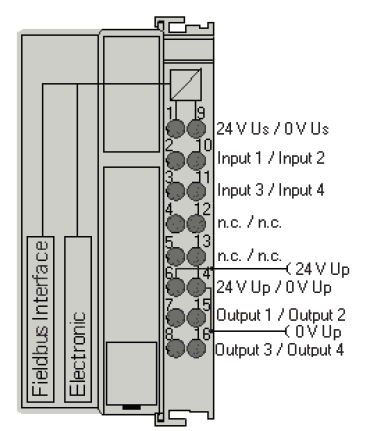
\includegraphics[scale=0.6]{Immagini/Sperimentale/Beckoffschema.PNG}
		\caption{Schema modulo bechoff}
		\label{fig:ModuloBechoff}
	\end{center}
\end{figure}
\subsubsection{Configurazione della rete}
La configurazione della rete prevede alla base il PC Target, in questo vi è una chiavetta USB che fa \textit{runnare} sul pc un sistema operativo simulink real time. Il target è il master della rete, ha due uscite ethernet, la prima è collegata direttamente al modulo bechkoff, il quale prende l'identità di primo slave, e come abbiamo visto precedentemente, al bechkoff sono attaccati e i due azionamenti che si comportano come slave aggiuntivi slave.
\begin{figure}[ht]
\begin{center}
    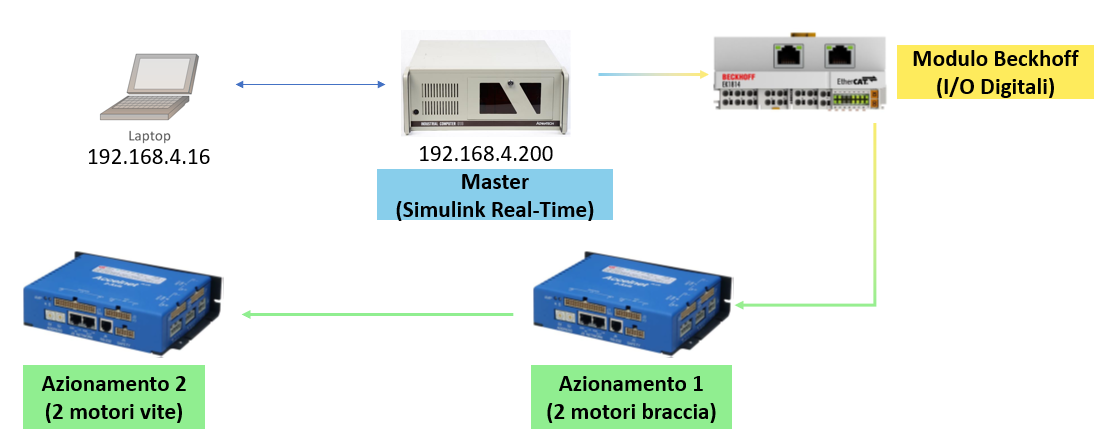
\includegraphics[scale=0.5]{Immagini/Sperimentale/Topology.PNG}
    \caption{Topologia della rete}
    \label{fig:NetTopology1}
\end{center}
\end{figure}
Invece, alla seconda porta ethernet, vi è collegato il PC dell'utente, il quale provvede a generare, compilare, e caricare ed  i programmi sul PC target. Da User-PC è anche possibile vedere i grafici e fare delle analisi sui movimenti e le traiettorie eseguite dal manipolatore. La connessione avviene tramite una rete ethernet, l'indirizzo del target è 192.168.4.200, invece per User-PC:
\begin{figure}[ht]
\begin{center}
    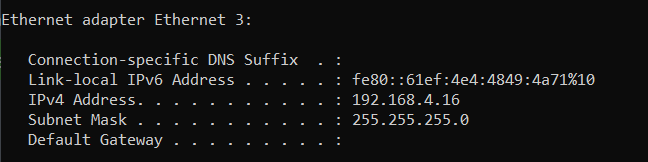
\includegraphics[scale=0.7]{Immagini/Sperimentale/ConfEthernet.png}
    \caption{Configurazione rete ethernet user PC}
    \label{fig:ConfEthernet}
\end{center}
\end{figure}
Va precisato che il pc dell'utente non fa parte della rete ethercat, ma la rete inizia soltanto dal pc target in poi, infatti, ad esclusione delle operazioni viste prima il manipolatore non ha bisogno del pc utente per funzionare.
\begin{figure}[ht]
	\begin{center}
		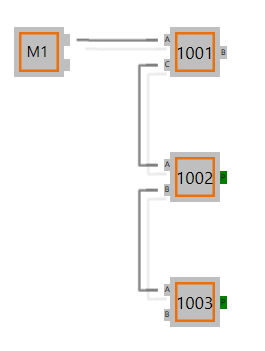
\includegraphics[scale=0.7]{Immagini/Sperimentale/NetTopology.png}
		\caption{Topologia rete mediante Ec-engineer}
		\label{fig:NetTopology2}
	\end{center}
\end{figure}
Una volta configurata la rete, il passo successivo è stato quello della configurazione dei messaggi, come è stato anticipato nel capitolo precedente il metodo di comunicazione sono le PDO. Le PDO possono essere in input o in output, la differenza sta nel fatto che le primo sono PDO che gli azionamenti trasmettono al master, di conseguenza il master le riceve, quelle di output invece sono PDO che il master trasmette e che gli azionamenti ricevono. 
\\Nelle immagini seguenti sono elencate le PDO di input, in particolare:
\begin{itemize}
 	\item PDO1 e PDO2 contengono i parametri di posizione, velocità coppia effettiva e modalità operativa che vengono trasmesse dagli azionamenti
 	\item PDO3, contiene input generici che sono indipendenti dalla modalità operativa del motore, in particolare è presente il \textit{general purpose inputs} che è il registro che permette la visione dei finecorsa
 	\item PDO4 contiene \textit{status word} e \textit{control word}, sono registri importanti che servono per verificare la modalità operativa e lo stato dell'azionamento, quindi sono utili per capire se l'azionamento è in fase pre-operativa, operativa o in errore
\end{itemize}
\begin{figure}[!ht]
\begin{subfigure}{.5\textwidth}
  \centering
  % include first image
  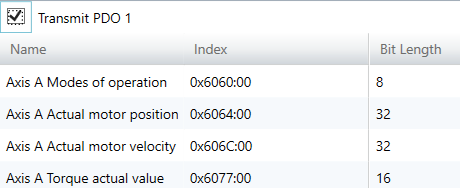
\includegraphics[width=.7\linewidth]{Immagini/Sperimentale/pdo1in.png}  
  \caption{PDO Input 1}
  \label{fig:sub-firstpdo}
\end{subfigure}
\begin{subfigure}{.5\textwidth}
  \centering
  % include second image
  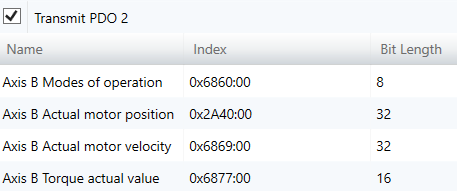
\includegraphics[width=.7\linewidth]{Immagini/Sperimentale/pdo2in.png}  
  \caption{PDO Input 2}
  \label{fig:sub-secondpdo}
\end{subfigure}
\begin{subfigure}{.5\textwidth}
  \centering
  % include third image
  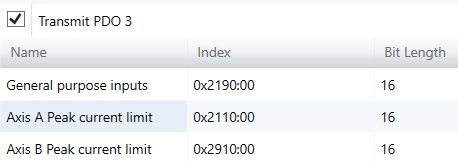
\includegraphics[width=.7\linewidth]{Immagini/Sperimentale/pdo3in.png}  
  \caption{PDO Input 3}
  \label{fig:sub-thirdpdo}
\end{subfigure}
\begin{subfigure}{.5\textwidth}
  \centering
  % include fourth image
  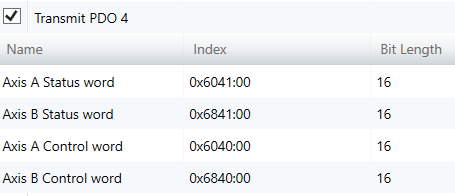
\includegraphics[width=.7\linewidth]{Immagini/Sperimentale/pdo4in.png}  
  \caption{PDO Input 4}
  \label{fig:sub-fourthpdo}
\end{subfigure}
\caption{PDO in input}
\label{fig:PDOIn}
\end{figure}
Per quanto riguarda le PDO che riceve l'azionamento sono solo due, ed i parametri ricevuti sono:
\begin{itemize}
	\item \textit{Modes of operation}, è un registro che specifica la modalità con la verrà controllato l'azionamento, per esempio coppia, posizione, velocità o ciclica
	\item \textit{Target torque}, specifica il valore di coppia che l'azionamento dovrà fornire al motore
\end{itemize}
\begin{figure}[ht]
\begin{center}
    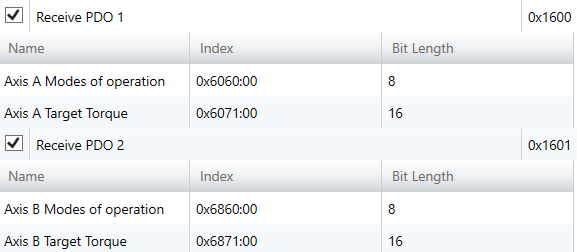
\includegraphics[scale=0.67]{Immagini/Sperimentale/pdo12out.png}
    \caption{PDO Output 1 e 2}
    \label{fig:PDOOut}
\end{center}
\end{figure}
\subsection{Implementazione nel sistema reale}
Una volta ottenuto il file ENI contenente la topologia della rete è stato utilizzato simulink real-time per implementare la logica di controllo del manipolatore
\begin{figure}[ht]
	\begin{center}
		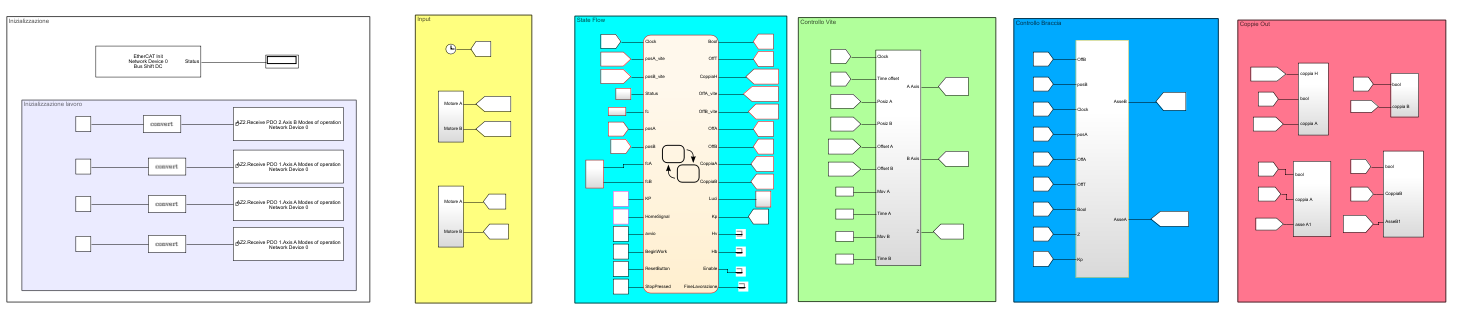
\includegraphics[scale=0.5]{Immagini/Sperimentale/generalSchema}
		\caption{Schema generale simulink}
		\label{fig:SimulinkSchema}
	\end{center}
\end{figure}
Il programma è stato diviso in sei stati diversi, andiamo ad analizzare ora i vari stati.
\subsubsection*{Inizializzazione}
\addcontentsline{toc}{subsubsection}{Inizializzazione}
La prima fase è quella di inizializzazione, in questa fase viene inserito il file ENI e viene specificata la modalità operativa degli azionamenti.
\begin{figure}[ht]
	\begin{center}
		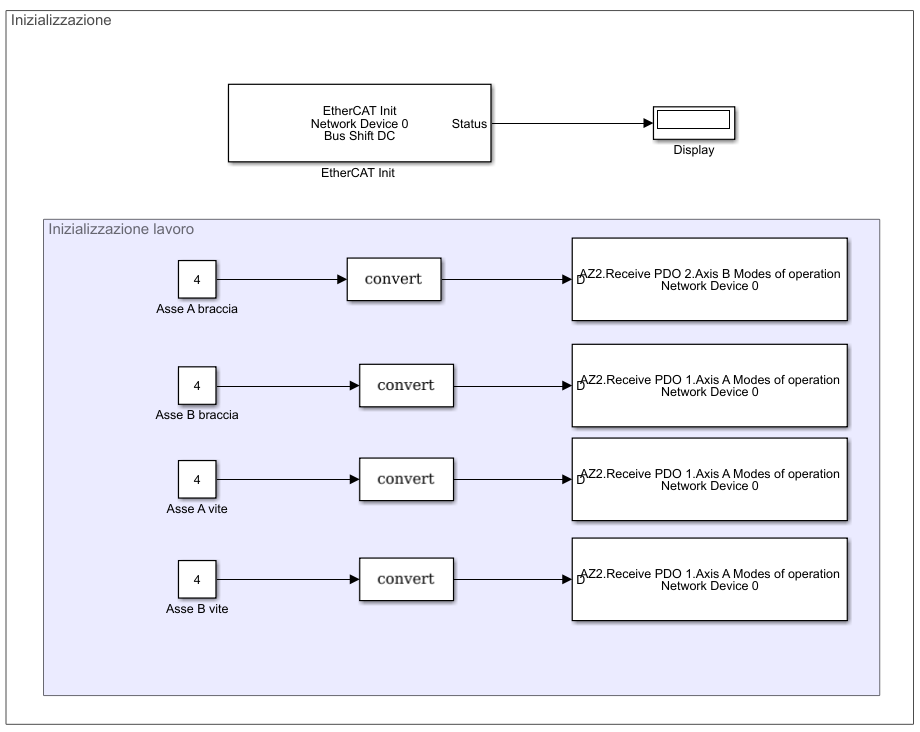
\includegraphics[scale=0.63]{Immagini/Sperimentale/Inizializzazione}
		\caption{Fase 1: Inizializzazione}
		\label{fig:Init}
	\end{center}
\end{figure}
Oltre al file ENI viene anche specificata la porta di comunicazione ed il bus che verranno utilizzati per lo scambio di dati. Ogni azionamento ha poi una determinata modalità operativa, come abbiamo visto nelle sezioni precedenti il controllo è effettuato in coppia. 
\begin{table}[h!]
	\centering
	\begin{tabular}{|c |c|} 
		\hline
		Modalità & Descrizione  \\ 
		\hline
		1 & modalità profilo in posizione  \\ 
		3 & modalità profilo in velocità  \\
		4 & modalità profilo in coppia   \\
		6 & modalità homing \\
		7 & modalità posizione interpolata\\
		\hline
	\end{tabular}
	\caption{Tipologie controllo azionamenti}
	\label{table:5}
\end{table}
\subsubsection*{Input}
\addcontentsline{toc}{subsubsection}{Input}
La seconda fase è quella di input, in questa fase andiamo a prendere tutti i valori di posizione dei motori sia della vite che delle braccia
\begin{figure}[ht]
	\begin{center}
		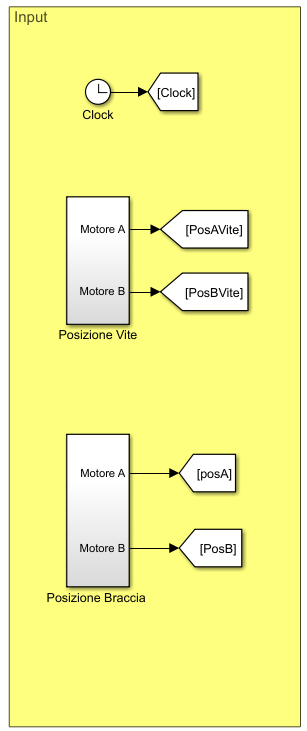
\includegraphics[scale=0.65]{Immagini/Sperimentale/Input}
		\caption{Fase 2: Input}
		\label{fig:Input}
	\end{center}
\end{figure}
I valori vengono presi mediante i messaggi dalle PDO ed hanno bisogno di essere convertiti, proprio per questo la struttura di ricezione di un messaggio è la seguente: 
\begin{figure}[ht]
	\begin{center}
		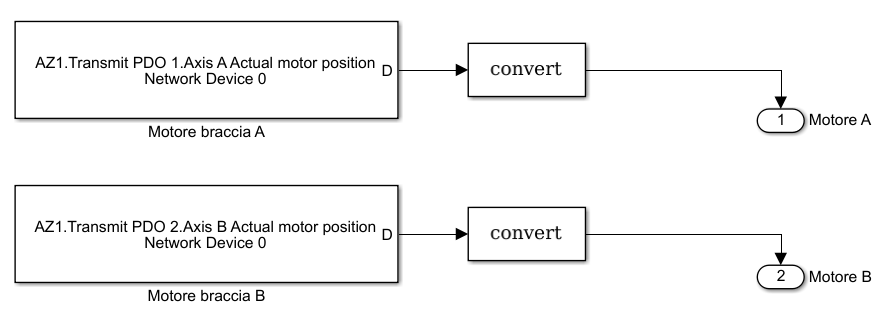
\includegraphics[scale=0.7]{Immagini/Sperimentale/convertS}
		\caption{Conversione e lettura motori}
		\label{fig:MotorConversion}
	\end{center}
\end{figure}
\subsubsection*{Stateflow}
\addcontentsline{toc}{subsubsection}{Stateflow}
Lo stateflow è un blocco dove viene posta la logica fondamentale dell'applicazione, in particolare in input avremo tutti i dati come ad esempio il clock, lo stato dei finecorsa, le posizioni dei motori e degli input che serviranno per l'interfaccia grafica. 
\begin{figure}[ht]
	\begin{center}
		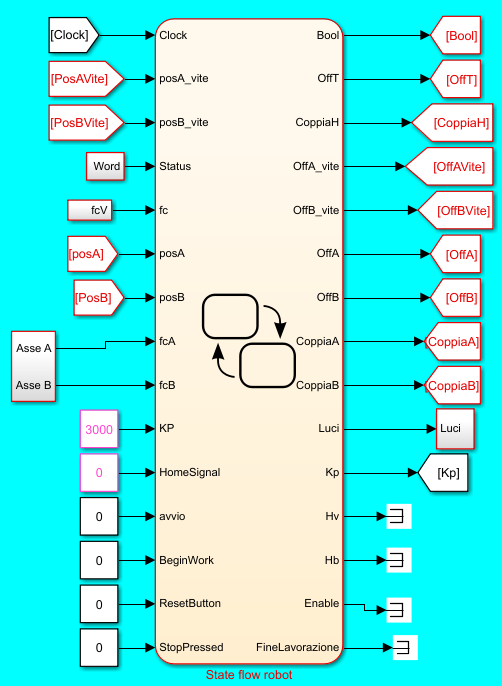
\includegraphics[scale=0.7]{Immagini/Sperimentale/sf0}
		\caption{Fase 3: Stateflow}
		\label{fig:Stateflow1}
	\end{center}
\end{figure}
In output invece abbiamo gli offset, che ci serviranno per capire di quanto ci siamo mossi nelle varie fasi, e quindi avere un riferimento sia di posizione che temporale, le coppie di homing dei motori e della vite, e un blocco relativo alla gestione delle luci\footnote{abbiamo la presenza di tre luci: rosso, bianco e verde, nei paragrafi successivi verrà introdotto il loro comportamento}.
\subsubsection*{Controllo vite}
\addcontentsline{toc}{subsubsection}{Controllo vite}
Il blocco Controllo Vite, contiene lo schema del controllore implementato per controllare la vite, in ingresso abbiamo il clock, le posizioni dei motori con relativi offset e la movimentazione da far eseguire ad entrambi i motori della vite con il tempo di esecuzione.
\begin{figure}[ht]
	\begin{center}
		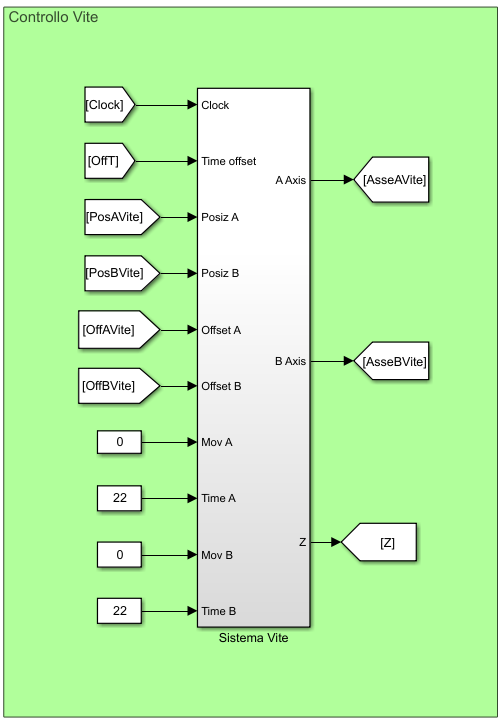
\includegraphics[scale=0.7]{Immagini/Sperimentale/ControlloViteSchema}
		\caption{Fase 4: Schema di controllo della vite}
		\label{fig:ControlloVite}
	\end{center}
\end{figure}
Grazie a tutti questi parametri potremo definire le leggi di moto che ci permetteranno il movimento nell'asse Z. Importante è sapere che il movimento eseguito dalla vite a ricircolo di sfere è dipendente anche dal movimento eseguito dalla guida lineare, infatti la rotazione provoca anche un abbassamento della vite, per risolvere questo problema il motore della guida dovrà essere sempre pronto a rispondere e correggere questa situazione; in caso che i due motori vadano alla stessa velocità si avrà una rotazione senza traslazione.
\subsubsection*{Controllo braccia}
\addcontentsline{toc}{subsubsection}{Controllo braccia}
Il blocco Controllo Braccia è quello responsabile della movimentazione dei link motorizzati, come per il blocco della vite prende in ingresso le posizioni, il \textit{clock} con i relativi offset e dentro vengono svolte le operazioni di generazione della legge di moto e di controllo. In uscita avremo le coppie che saranno assegnate ai due assi.
\begin{figure}[ht]
	\begin{center}
		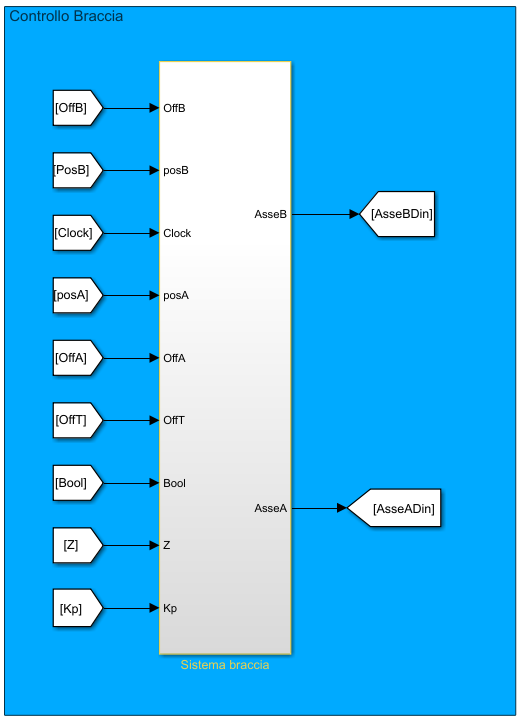
\includegraphics[scale=0.75]{Immagini/Sperimentale/ControlloBraccia}
		\caption{Fase 5: Schema di controllo delle braccia}
		\label{fig:controlloBraccia}
	\end{center}
\end{figure}
\subsubsection*{Coppie uscita}
\addcontentsline{toc}{subsubsection}{Coppie uscita}
Dopo aver ottenuto le coppie di homing dallo stateflow e le coppie dei motori dagli schemi di controllo è venuto il momento di inviare le coppie agli azionamenti e di conseguenza ai motori; per far questo usiamo un bloco per ogni motore, oltre alle coppie in entrata avremo anche una variabile di controllo. 
\begin{figure}[ht]
	\begin{center}
		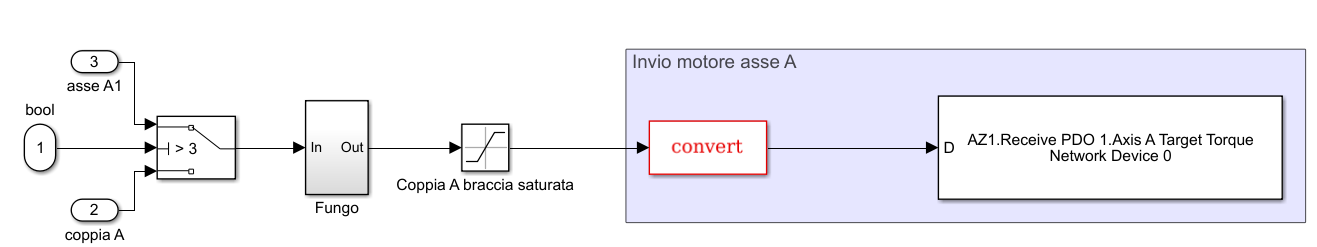
\includegraphics[scale=0.55]{Immagini/Sperimentale/Saturatore}
		\caption{Schema espanso invio coppia}
			\label{fig:CoppieoutExpanded}
	\end{center}
\end{figure}
Nella figura precedente è possibile vedere lo schema espanso come spiegato, lo switch permette la scelta in base alla variabile bool, fintanto che è minore o uguale a 3 verrà erogata solo la coppia di Homing, quando arriva a 4 invece vuol dire che siamo nella fase di controllo, di conseguenza verrà erogata la coppia di controllo. Successivo allo switch c'è un blocco che serve per la gestione delle emergenze, infatti, una volta premuto il fungo verrà assegnata una coppia costante uguale a 0 che fermerà la lavorazione ed anche dopo che verrà sbloccato il fungo la coppia per sicurezza rimarrà a zero, l'unico modo per resettare questa condizione è il riavvio del programma.
\begin{figure}[ht]
	\begin{center}
		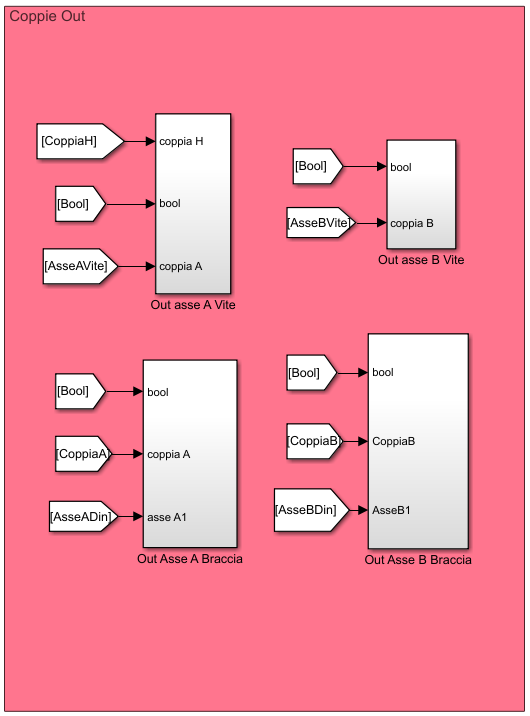
\includegraphics[scale=0.6]{Immagini/Sperimentale/CoppieOut}
		\caption{Fase 6: Copie in uscita
			\label{fig:Coppieout}}
	\end{center}
\end{figure}
\\Successivo al blocco fungo abbiamo un saturatore, questo serve per evitare di danneggiare il manipolatore in caso che le coppie computate siano molto alte, è stato trovato sperimentalmente un limite che coincide con la coppia nominale che non può essere superato, per concludere l'ultima parte è quella che si occupa di inviare mediante PDO il valore di coppia convertito all'azionamento.
\\Andiamo ora a concentrarci sulle parti principali di questo programma, in particolare andremo a trattare lo stateflow il metodo di funzionamento ed i vari stati, passeremo poi all'interfaccia grafica che permette di comandare il manipolatore, e per concludere andremo a vedere i controllori implementati per la vite e per le braccia, andando a vedere la struttura, lo schema e i risultati ottenuti per ogni approccio.
\subsection{Stateflow}
\textit{Stateflow} si occupa di fornire diagrammi di transizione, stato e di flusso utilizzando un linguaggio grafico. Nel caso del manipolatore è stato utilizzato per la progettazione di diagrammi di transizione in base agli stati del robot. In questa sezione andremo a vedere le fasi gli stadi di evoluzione che sono stati costruiti.
\subsubsection{Fase di Homing}
Appena il robot viene acceso non possiamo sapere dove si trova, di conseguenza abbiamo bisogno di uno stadio che ci vada a trovare una posizione di riferimento nella quale sappiamo dove è collocato effettivamente. Il primo stadio è quindi quello di \textit{homing}, consiste nel portare i motori a toccare i finecorsa indicandogli che quello è il loro punto di partenza. I motori utilizzati per questa fase sono stati quelli delle braccia e quello di traslazione della vite.
\\L'approccio iniziale è stato quello di fornire una coppia costante che in automatico si occupava di andare a toccare i finercorsa, e dopo che li toccava si passava nello stato successivo. Però, per motivi di sicurezza e considerando che lasciando fermo il manipolatore per diverso tempo la stessa coppia magari potrebbe non farlo muovere si è deciso di chiudere l'anello in posizione, in particolare per eseguire la fase di homing è stata data una rampa con pendenza negativa in quanto i finecorsa vengono rilevati quando i link sono totalmente a destra.
Per controllare questa rampa è stato fatto un controllo proporzionale e integrale sull'errore tra la posizione attuale ed il riferimento, la legge implementata è quindi del tipo:
\begin{equation*}
	PI = \frac{K_p s + K_i}{s}
\end{equation*}
Nella figura successiva andiamo a vedere lo schema effettivamente implementato per questa prima fase:
\begin{figure}[ht]
\begin{center}
    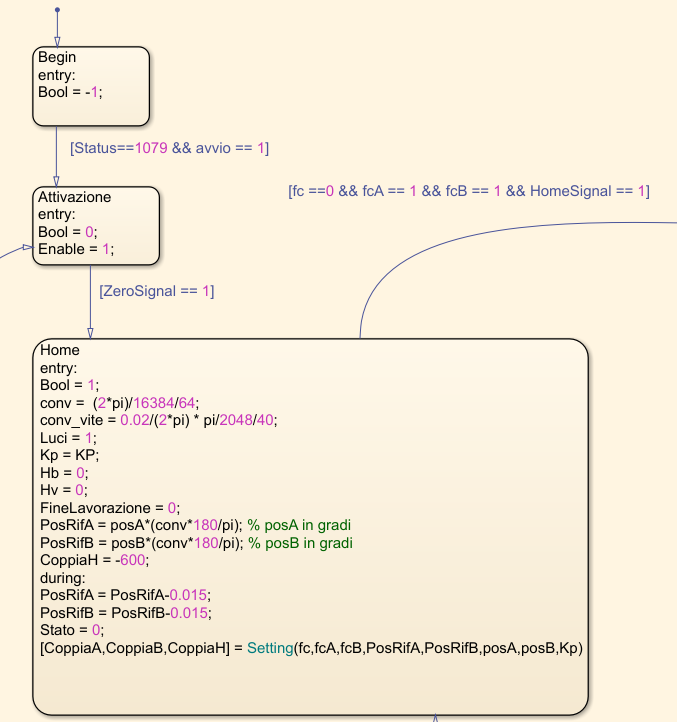
\includegraphics[scale=0.8]{Immagini/Sperimentale/state1new.png}
    \caption{Fase di Homing}
    \label{fig:Zero}
\end{center}
\end{figure}
\\Il primo stato è quello di begin, appena il programma si avvia ci entriamo in automatico, per passare allo stato successivo, ovvero attivazione abbiamo bisogno di due condizioni, la prima si verifica quando la \textit{Status Word} è uguale a 1079, ovvero quando gli azionamenti sono usciti dalla fase \textit{pre-operational} e sono quindi pronti all'uso, la seconda condizione invece è quando il segnale avvio è vero, nello stato attivazione i motori sono ancora fermi però viene abilitato il loro utilizzo, passare quindi in questo stato è obbligatorio. Per passare allo stato successivo il segnale \textit{ZeroSignal} deve essere vero, questo è un segnale gestito mediante un bottone da interfaccia grafica, appena viene premuto entriamo nello stato \textbf{Home}. In questo stato vengono definite variabili per la conversione dei valori\footnote{I valori presi dai motori sono espressi tutti in conti, per quello è stata necessaria una fase di analisi dei motori per capire come convertirli, successivamente c'è stato un passaggio da counts a radianti e da radianti a gradi.}, viene poi salvata la posizione di riferimento dell'asse A e B dei motori delle braccia. La fase successiva è quella del \textit{during}, rimanendo in quello stato quella fase viene eseguita ad ogni ciclo (1ms), in questa abbiamo la rampa che decresce di 0.015 gradi al millisecondo (15 gradi al secondo) e abbiamo una funzione simulink che è quella che si occupa del controllo PI. Una volta raggiunta la posizione del finecorsa le coppie vengono settate a 0, impedendo quindi un'ulteriore movimentazione. Per passare alla fase successiva abbiamo bisogno che tutti gli elementi siano arrivati a finecorsa.
\subsubsection{Fase di posizionamento}
La fase successiva è quella di posizionamento, per non lasciare il robot nella configurazione di zero si è scelto di spostarlo in una configurazione standard lontana dai punti di singolarità e che sarà comoda per le movimentazioni e traiettorie successive. La configurazione scelta prevede che i giunti siano messi a $100^\circ$ e $80^\circ$, anche qua come prima il primo approccio è stato quello di utilizzare una coppia costante per il movimento; la fase di zero lasciava i link a $60^\circ$ e $-30^\circ$, vi era quindi la necessità di fare $+40^\circ$ per il motore a sinistra e $+110^\circ$ per il motore a destra, la coppia costante veniva erogata finché non si arrivava a quelle condizioni, dopodiché eravamo sicuri che il posizionamento era stato fatto in maniera corretta. La vite invece ha due modalità di configurazione, è possibile farla abbassare o lasciarla alta in finecorsa, si è scelto di proseguire in questo modo in quanto alla vite come abbiamo visto precedentemente è possibile collegare degli utensili e quindi l'abbassamento la predisponeva al disegno per traiettorie bidimensionali. L'approccio di controllo finale però non è stato quello della coppia costante, anche in questo caso per motivi di sicurezza ma, sapendo le posizioni finali che si volevano raggiungere, si è optato per definire una legge di moto che si occupa di portarci nella condizione di posizionamento desiderata
\begin{figure}[ht]
\begin{center}
    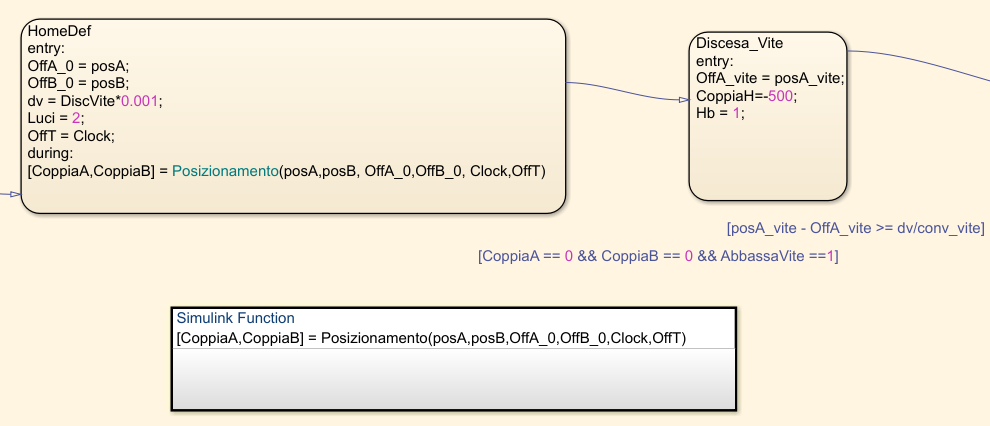
\includegraphics[scale=0.7]{Immagini/Sperimentale/state2New.png}
    \caption{Fase di posizionamento}
    \label{fig:Pos}
\end{center}
\end{figure}
\\Riprendendo lo schema precedente, per passare allo stato \textbf{HomeDef} bisogna aver raggiunto tutti i finecorsa; non appena entriamo vengono salvati gli offset della posizione delle braccia, del tempo e la posizione desiderata di discesa della vite. Ad ogni ciclo, quindi ogni millisecondo viene eseguita la funzione \textbf{Posizionamento($\dots$)} la quale, mediante una legge di moto, ci consente di eseguire in maniera corretta il posizionamento.
Andando ad analizzare nello specifico il blocco simulink del posizionamento, vengono costruite due leggi polinomiali, una per ogni motore che forniscono un \textit{setpoint} in posizione in gradi, che verrà confrontato con la posizione attuale. Per ottenere poi una coppia, e garantire errore a transitorio esaurito viene introdotto un sistema di controllo proporzionale integrativo, con legge di controllo: 
% check formula
\begin{equation*}
\tau = K \tilde{\theta} = \begin{bmatrix}
K_p & K_p \\ K_i & K_i
\end{bmatrix}
\begin{bmatrix}
\tilde{\theta_1} \\ \tilde{\theta_2}
\end{bmatrix} = K_p\theta + K_i\theta
\end{equation*}
Le coppie di controllo uscenti andranno quindi al manipolatore e si occuperanno della movimentazione. Possiamo vedere lo schema della legge di moto implementato in figura \ref{fig:ImpPos}.
\begin{figure}[ht]
	\begin{center}
		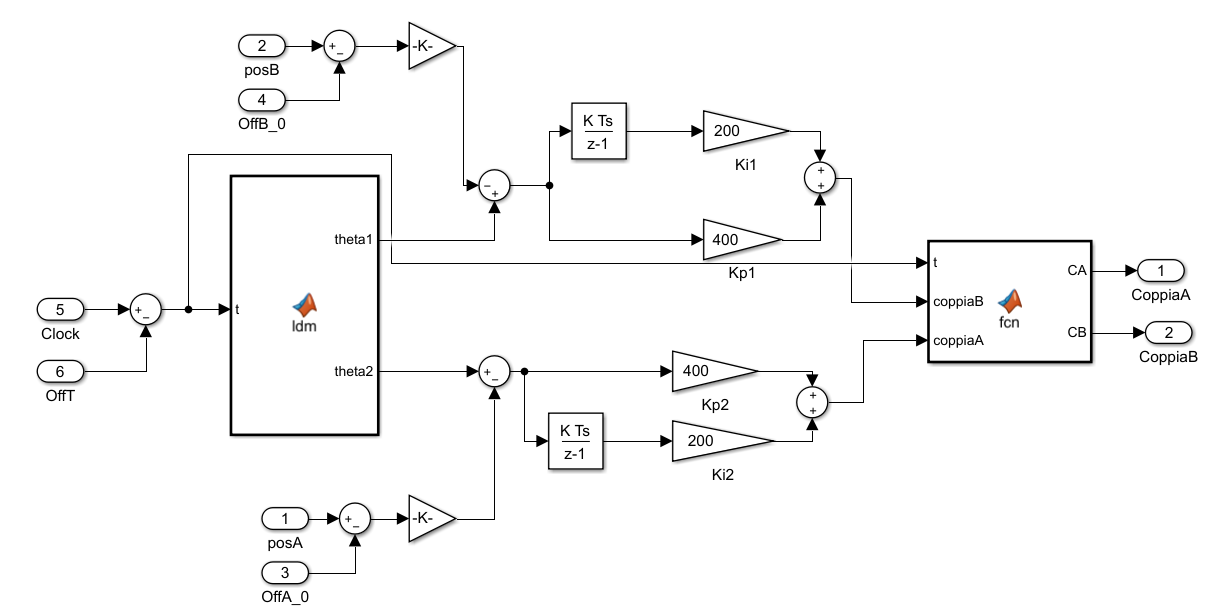
\includegraphics[scale=0.6]{Immagini/Sperimentale/LdmPosizionamento}
		\caption{Implementazione funzione di posizionamento}
		\label{fig:ImpPos}
	\end{center}
\end{figure}
\par Una volta eseguito il posizionamento, lo stato successivo riguarderà la discesa della vite, per passarci le coppie dei bracci dovranno essere pari a zero e sull'interfaccia grafica dovrà essere premuto il bottone relativo alla discesa. In particolare per la discesa verrà utilizzata la variabile \textbf{dv} salvata precedentemente che indica di quanti centimetri la vite deve scendere; per farla scendere verrà fornita una coppia al motore di traslazione che si occuperà di arrivare alla posizione desiderata.
\subsubsection{Fase di controllo}
L'ultima fase è quella di controllo ed esecuzione della traiettoria, in questa fase andiamo a settare l'offset dei motori della vite, del tempo e dei motori delle braccia, serve resettare l'offset della vite in quanto il posizionamento (nel caso di discesa) è stato appena concluso; l'offset del tempo ci permette di far partire virtualmente il tempo da zero negli schemi di controllo dopo che siamo arrivati alla configurazione di \textit{Homing}.
\begin{figure}[ht]
\begin{center}
    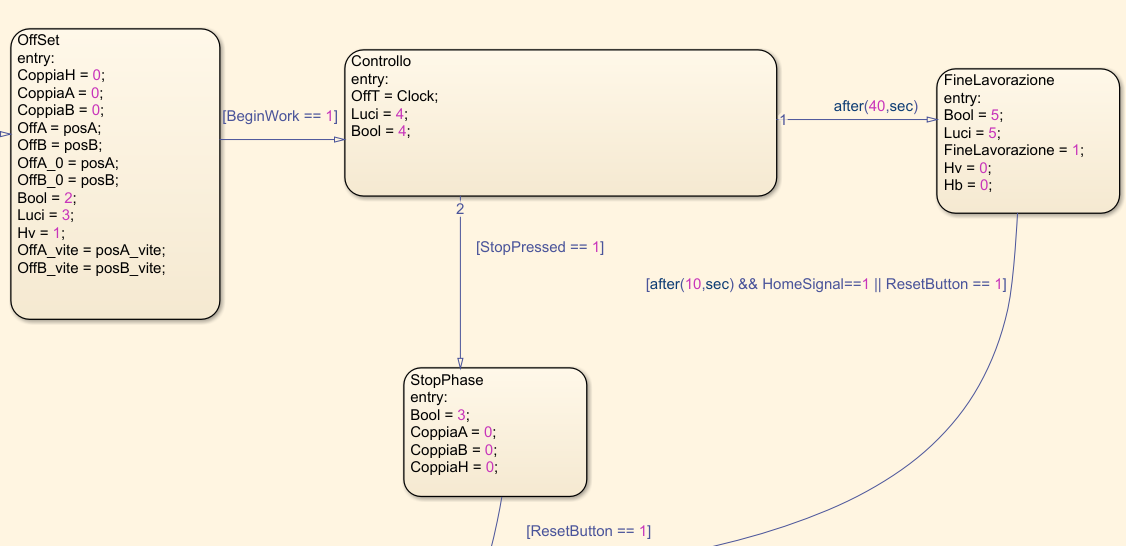
\includegraphics[scale=0.6]{Immagini/Sperimentale/state3New.png}
    \caption{Fase di controllo}
    \label{fig:Traiettoria}
\end{center}
\end{figure}
Come abbiamo anticipato precedentemente nello stato \textbf{OffSet} c'è il settaggio degli \textit{offset} e tutte le coppie vengono messe a zero per evitare eventuali movimentazioni indesiderate. Per passare alla fase successiva abbiamo bisogno che venga premuto il bottone \textbf{Work} sull'interfaccia grafica, questo garantirà il passaggio allo stato \textit{Controllo}, può darsi che il bottone non venga premuto subito, di conseguenza il clock potrebbe aumentare, per questo l'offset del clock viene settato nella fase di controllo. Per quanto riguarda la scelta della traiettoria tramite interfaccia grafica vi è la possibilità di scegliere quella desiderata. A livello implementativo le traiettorie non sono altro che leggi di moto fatte in due o tre dimensioni, dipendentemente dal caso, dopo che il manipolatore inizia ad eseguire la traiettoria possono esserci due evoluzioni:
\begin{itemize}
	\item la traiettoria viene eseguita correttamente
	\item la traiettoria da problemi
\end{itemize}
Nel primo caso abbiamo 40 secondi per eseguire la traiettoria (il tempo può essere personalizzato in base alla tipologia di traiettorie), alla fine di questo tempo passiamo allo stato \textbf{FineLavorazione} dove il manipolatore è fermo ed ha concluso la sua traiettoria, da questo mediante il bottone di reset è possibile ritornare alla fase di zero, oppure in automatico dopo un determinato periodo di tempo se il tasto di homing è stato lasciato attivo il manipolatore torna all'homing. Nel secondo caso ci si accorge che la traiettoria sta dando problemi, magari vibrazioni o si vede che il manipolatore rischia di entrare in singolarità, per prevenire questo vi è un bottone denominato \textbf{STOP} che permette l'arresto immediato del manipolatore, azzerando tutte le coppie. A differenza della pressione del fungo, che dopo lo sbloccaggio richiede il riavvio del dispositivo, nel caso in cui si entri nella fase di stop mediante il bottone di reset è possibile far tornare il manipolatore nella fase di attivazione, da questa poi sarà possibile far partire di nuovo la fase di zero e successivamente quella di homing.

\subsubsection*{Gestione variabile di stato e luci}
\addcontentsline{toc}{subsubsection}{Gestione variabile di stato e luci}
Durante tutte le fasi è possibile vedere nello stateflow che due variabili si evolvono costantemente: bool e luci; la prima serve per indicare lo stato nel quale si trova il manipolatore, in particolare è state definita la seguente tabella degli stati.
\begin{table}[h!]
\centering
\begin{tabular}{|c |c |} 
 \hline
 Valore & Stato \\ [0.5ex] 
 \hline\hline
  -1  & Pre-operativo \\ 
  0  & Attivo \\
  1 & Homing \\
  2 & Manipolatore posizionato\\
  3 & Traiettoria\\
  4 & Manipolatore fermo\\
 \hline
\end{tabular}
\caption{Valori variabile \textit{bool}}
\label{table:3}
\end{table}
\\La seconda invece serve a pilotare le luci in modo tale da avere un feedback visuale che indica fase in cui è il manipolatore.
\begin{table}[h!]
\centering
\begin{tabular}{|c |c|c|} 
 \hline
 Valore & Colore & Bool \\ [0.5ex] 
 \hline\hline
  1  & Bianco & 1 \\ 
  2 &  Bianco Rosso & 1\\
  3 &  Rosso & 2 \\
  4 & Bianco Verde & 3\\
  5 & Verde & 4\\
 \hline
\end{tabular}
\caption{Valori luci}
\label{table:luci}
\end{table}
\subsubsection{Interfaccia grafica}
Per gestire al meglio le varie impostazioni, e per essere sicuri del passaggio tra i vari stati è stata creata un'interfaccia grafica \textit{user-friendly} mediante \textit{instrument panel} fornito da \textit{Simulink real-time explorer}
\begin{figure}[ht]
	\begin{center}
		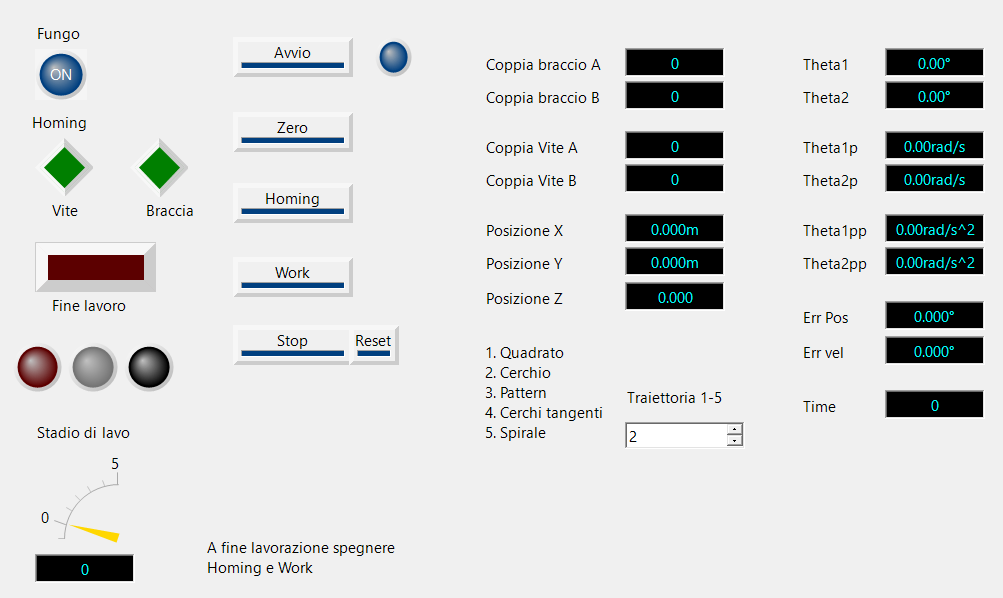
\includegraphics[scale=0.6]{Immagini/Sperimentale/GUI2}
		\caption{Interfaccia grafica}
		\label{fig:gui}
	\end{center}
\end{figure}
\\A sinistra, dall'alto in basso possiamo vedere dei LED che hanno la funzionalità di:
\begin{itemize}
	\item Fungo: rimane acceso fintantoché il fungo non è premuto
	\item Homing: si accendono quando i motori hanno raggiunto il finecorsa
	\item Fine lavoro: appena la traiettoria assegnata finisce questo si accende
	\item Luci: sono i led visti nella tabella \ref{table:luci}, che vanno ad indicare in che fase di lavoro è il manipolatore, per comodità visiva il led bianco nell'interfaccia è stato sostituito da uno ocra
\end{itemize} 
Sotto questi led abbiamo un indicatore che va a specificare le fasi di lavoro come viste nella tabella \ref{table:3}. Al centro abbiamo i bottoni che permettono di passare tra le varie fasi dello stateflow e di fare tutte le operazioni quindi avvio, zero, homing, lavoro stop e reset. In particolare i bottoni funzionano tramite il collegamento ad una variabile, e quelle di riferimento sono le ultime costanti collegate in input allo stateflow visto in figura \ref{fig:Stateflow1}. A destra abbiamo invece una parte di visualizzazione dove vediamo tutti i parametri di interesse del manipolatore, in particolare le coppie fornite e le posizioni sia nel piano $[x,y,z]$ che quelle ai link motorizzati quindi $\theta_1,\theta_2$. Infine, abbiamo il selettore di traiettoria, il quale permette la scelta fra le sei opzioni possibili (di default viene eseguito il cerchio).
\begin{enumerate}
	\item Quadrato
	\item Cerchio
	\item Pattern
	\item Cerchi tangenti
	\item Spirale
	\item Solo asse Z
\end{enumerate}
Adesso che abbiamo introdotto la logica di funzionamento a stati, proseguiamo la nostra trattazione andando a vedere le tipologie di controllo che sono state implementate, in particolare inizieremo col guardare il controllo applicato alla vite e successivamente quello per le braccia.
\subsection{Controllo vite}%CHECK
Lo scopo di questa sottosezione è quello di introdurre le due tipologie di controllo per la vite, da un punto di vista teorico e andare ad analizzare il comportamento pratico. Il sistema, essendo formato da due parti, e potendo fare solo due movimenti è ad un solo grado di libertà non risulta essere quindi molto complesso. Gli approcci di controllo utilizzati sono di tipo centralizzato, l'analisi di questi controllori verrà fatta mediante funzioni di trasferimento, proseguire con andiamo quindi ad introdurre la legge di controllo di un controllore PID generico:
\begin{equation}
\tau_v (t) = K_p \bigg(q_v(t) + \frac{1}{T_I} \int_0^t q_v(\tau) d\tau + T_D \frac{d q_v(t)}{dt}\bigg)
\label{eq:PID}
\end{equation}
\subsubsection{Controllo proporzionale}
Il primo controllo implementato è quello proporzionale, questa tipologia di controllo si basa sull'idea che ingresso ed uscita siano legati in modo algebrico da un coefficiente $K_p$ chiamato anche guadagno proporzionale. La legge di controllo è quindi definita come
\begin{equation}
\tau_v = K_p q_v
\end{equation}
\begin{figure}[ht]
	\begin{center}
		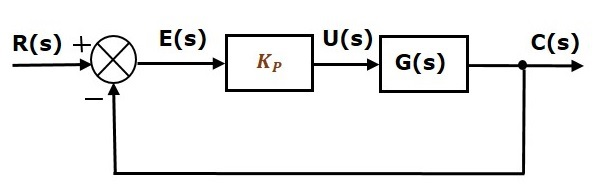
\includegraphics[scale=0.6]{Immagini/Controllori/Pschema}
		\caption{Schema teorico controllore proporzionale}
		\label{fig:Pschema}
	\end{center}
\end{figure}
L'azione proporzionale è utile in quanto più grande è l'errore all'ingresso del controllore e maggiore sarà l'azione svolta da esso. Il regolatore, riprendendo l'equazione \ref{eq:PID} si può notare che solo con il contributo proporzionale la velocità di risposta del sistema aumenta, però con guadagno elevato diminuisce la stabilità e quindi aumentano le oscillazioni\footnote{Il parametro proporzionale viene definito ed analizzato molto in letteratura, nella pratica però è solo un parametro teorico, infatti solitamente ci si riferisce alla banda proporzionale, definita come la variazione minima dell'ingresso che porta l'uscita al valore minimo percentuale.}.
Andiamo ora a vedere l'implementazione del controllore:
\begin{figure}[ht]
	\begin{center}
		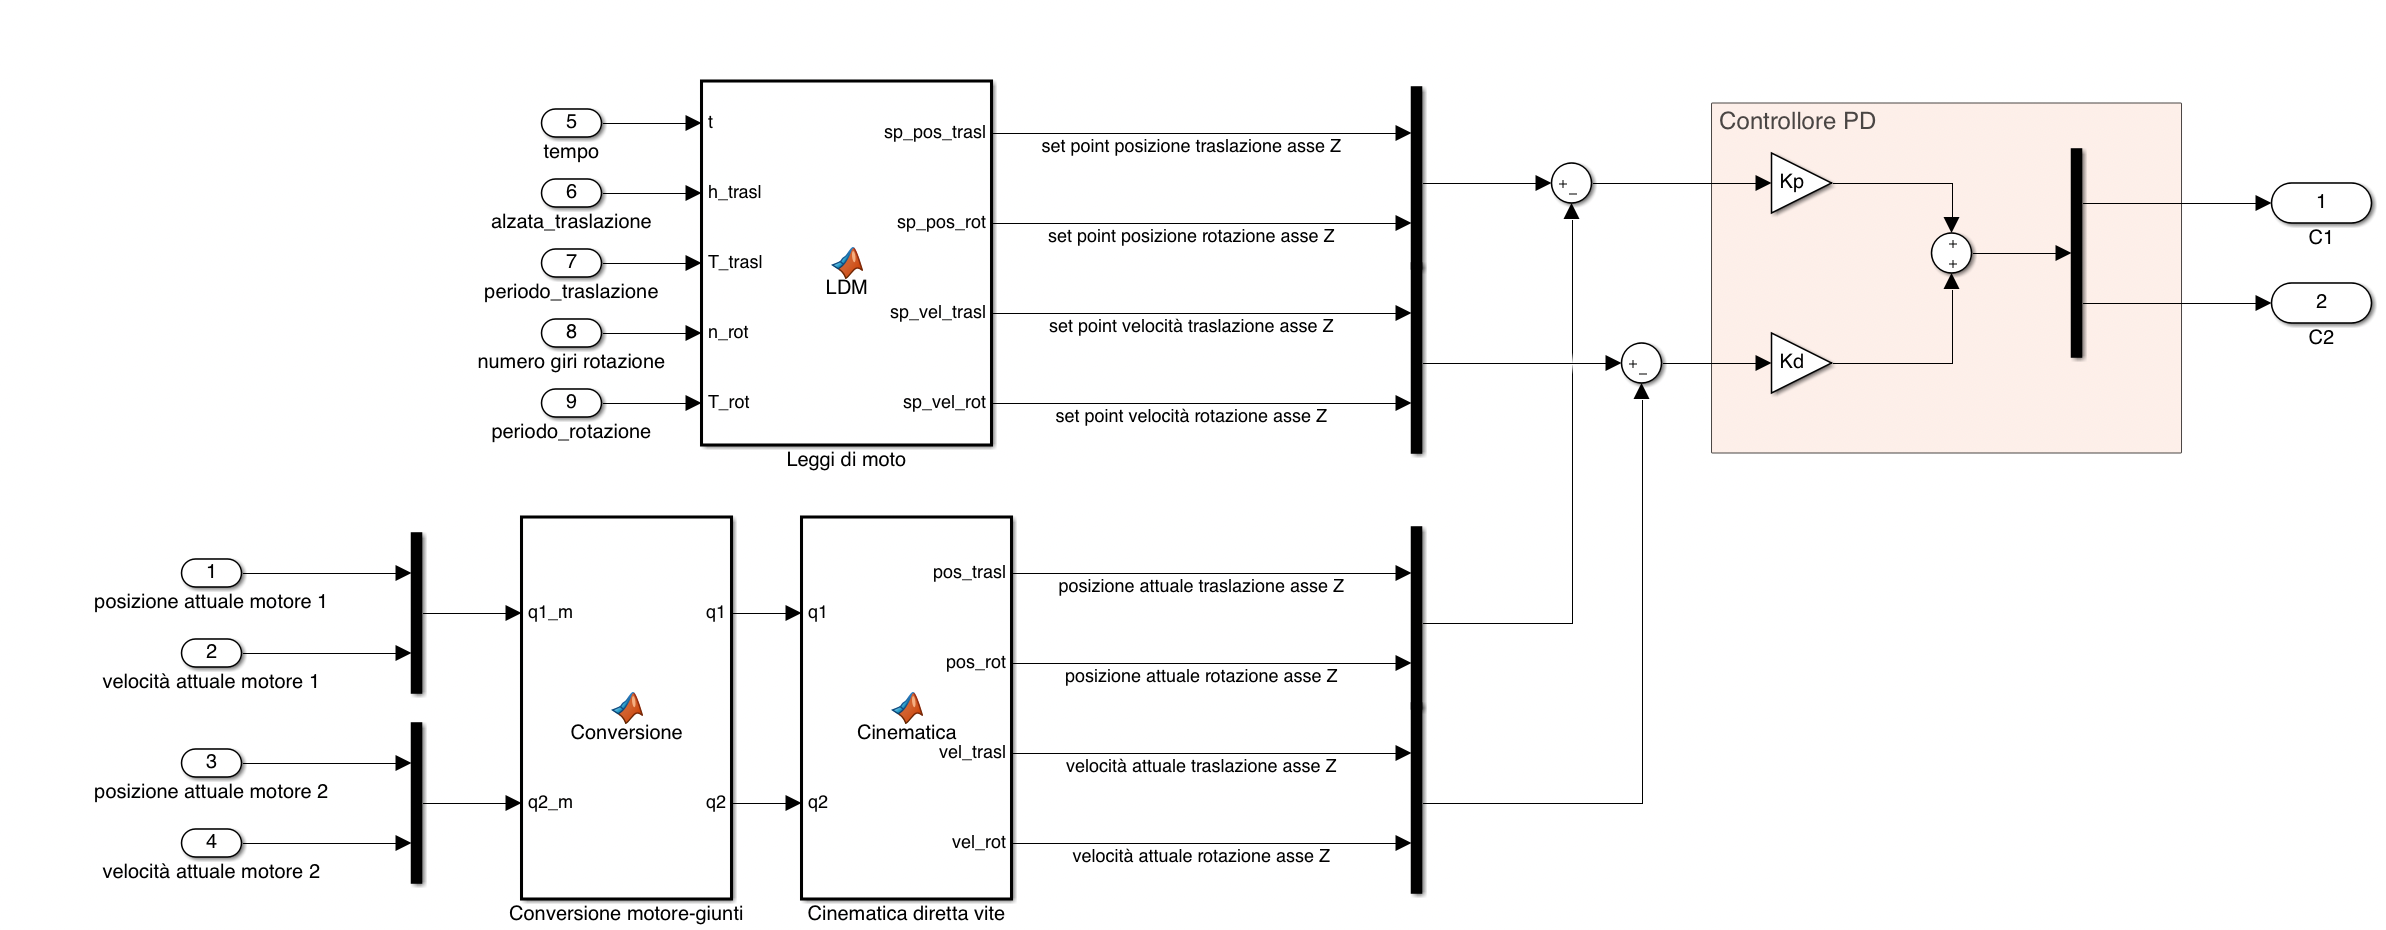
\includegraphics[scale=0.37]{Immagini/Controllori/Vite}
		\caption{CAMBIARE}
		\label{fig:PVite}
	\end{center}
\end{figure}
INSERIRE DESCRIZIONE E ALTRO
\subsubsection{Controllo proporzionale derivativo}
A partire dal controllore precedente andiamo ad aggiungere una parte: l'azione derivativa. In uscita fornisce la derivata rispetto al tempo dell'errore, se dovessimo analizzarla singolarmente potremmo definire una legge del tipo:
\begin{equation}
\tau_v = K_D\dot{q}_v
\end{equation}
Abbiamo la presenza della velocità, infatti il controllore derivativo viene anche chiamato controllore di velocità, il suo comportamento è sostanzialmente diverso da quello proporzionale in quanto l'uscita dipende dalla velocità con la quale varia l'errore e riesce a fornire un anticipo di fase. Riprendendo l'equazione \ref{eq:PID} il parametro che controlla questo anticipo è $T_D$ infatti nel caso in cui $K_P=K_I=0$ andando ad analizzare solo il suo comportamento si nota che la stabilità del sistema peggiora sia aumentando che diminuendo il valore. Andando ora ad unire i due contributi otteniamo un controllore PD.
\begin{figure}[ht]
	\begin{center}
		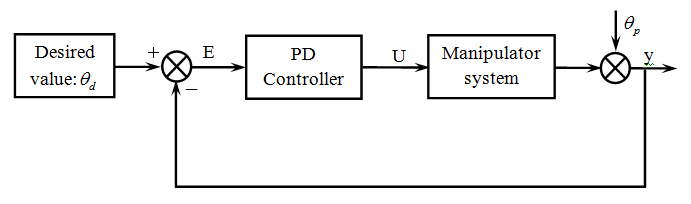
\includegraphics[scale=0.35]{Immagini/Controllori/PDSchema}
		\caption{Schema teorico controllore PD }
		\label{fig:PDSchema}
	\end{center}
\end{figure}
Possiamo scrivere l'azione combinata dei due controllori considerando il rapporto ingresso uscita e ottenendo:
\begin{equation}
\tau_v = K_P(1+sT_D)
\end{equation}
con $T_D = \frac{K_D}{K_P})$. In caso di ingresso definito come uno scalino, la presenza del termine derivativo va ad introdurre uno zero e ad aumentare il coefficiente di s, andando a ridurre le oscillazioni e di conseguenza stabilizzando il sistema. Andiamo ora a vedere l'implementazione sul manipolatore del controllore PD:
\begin{figure}[ht]
	\begin{center}
		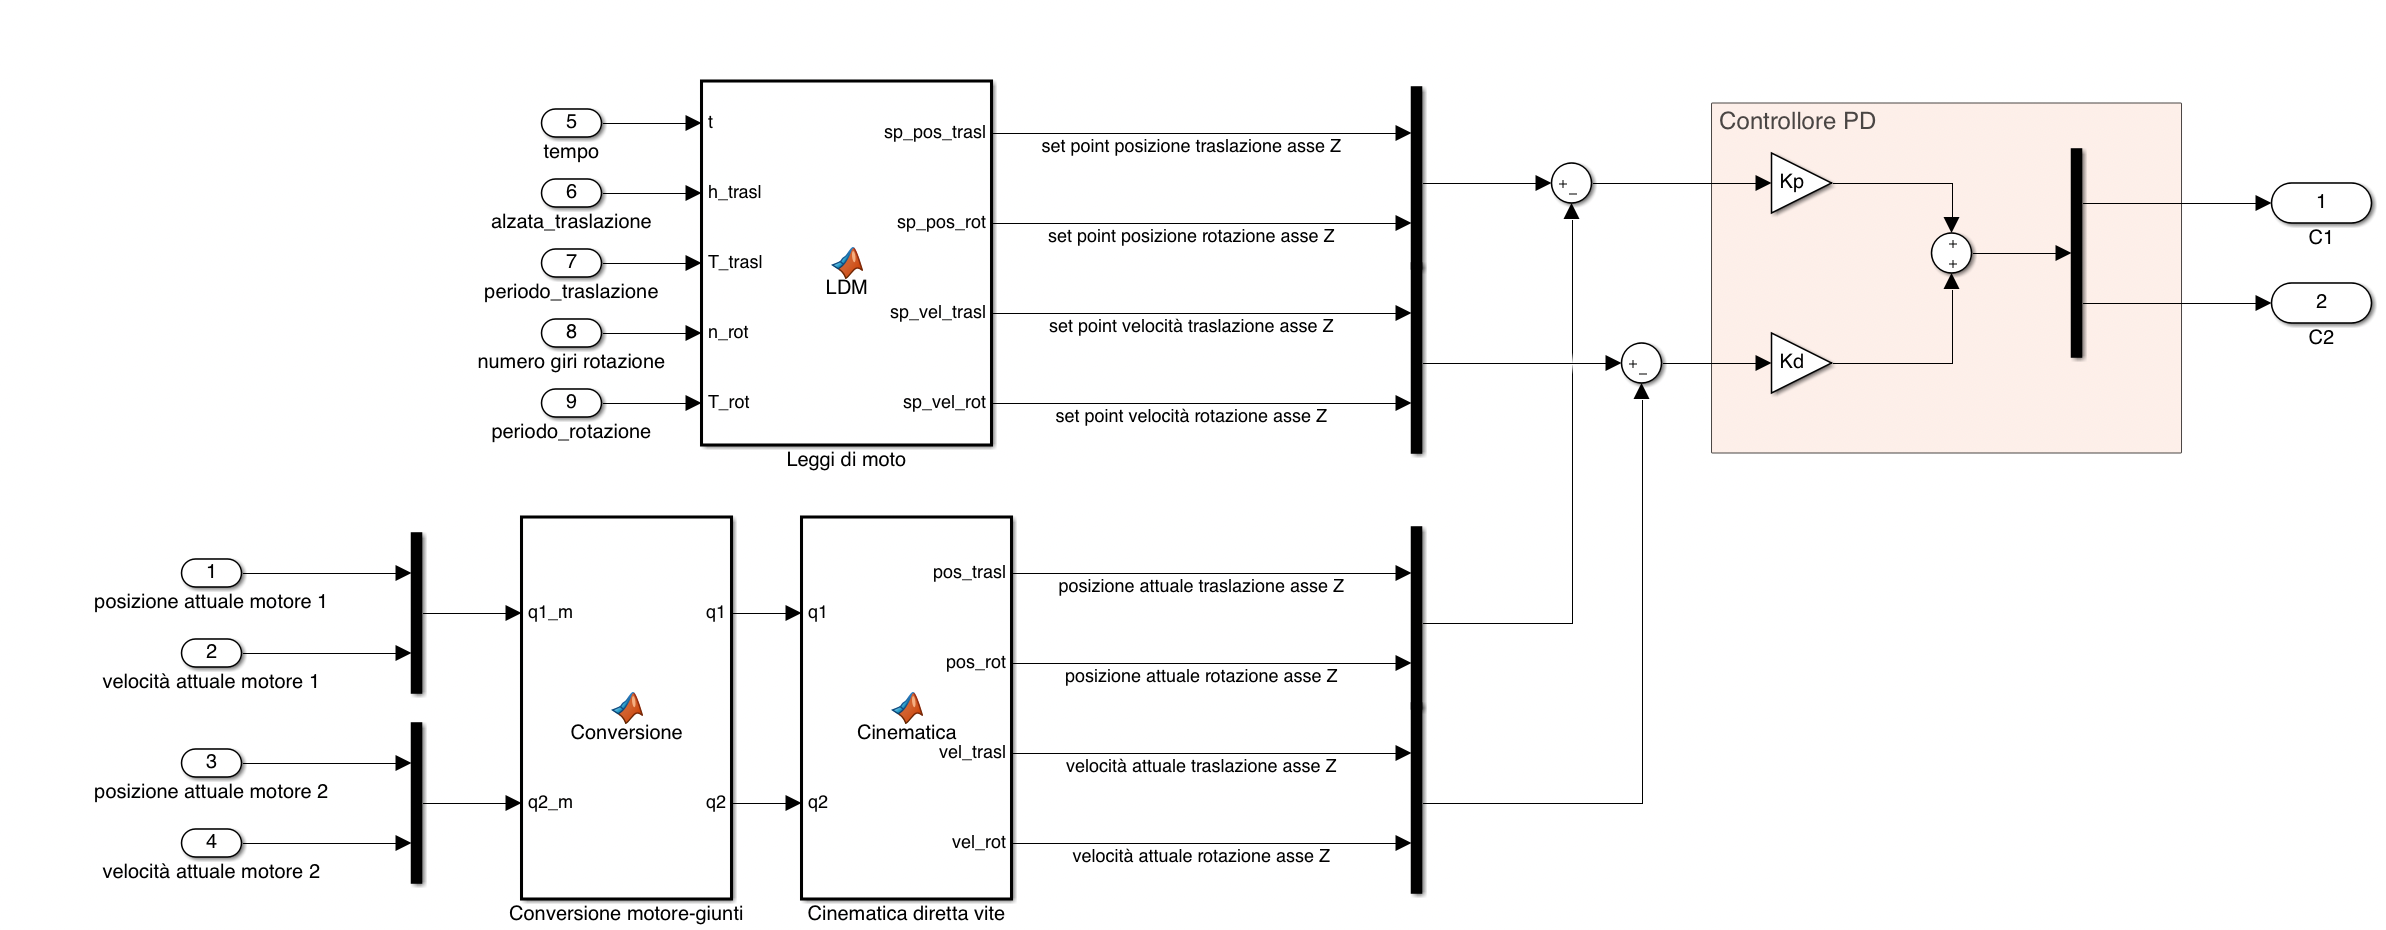
\includegraphics[scale=0.35]{Immagini/Controllori/Vite}
		\caption{Controllore PD Vite}
		\label{fig:PDVite}
	\end{center}
\end{figure}
A partire da una legge di moto per entrambi i motori che fornisce quattro set point, abbiamo: una prima fase di raccolta dei dati nei quali si prendono le posizioni e velocità dei motori della vite, essendo i motori connessi a riduttori, ed operando sui giunti abbiamo un blocco che si occupa di fare la conversione; una volta fatta la conversione vi è la necessità di effettuare la cinematica diretta per poter passare dagli angoli alle coordinate dell'asse z. In seguito verrà fatta una differenza tra le posizioni e velocità ottenute con la cinematica e quelle del \textit{set-point}; gli errori verranno poi moltiplicati per $K_P$ (posizione) e $K_D$ (velocità) per ottenere i valori della legge di controllo da assegnare ai motori.
\\INSCERISCI CONFRONTI ETC
\subsection{Controllo braccia}
Questa sottosezione si pone come obiettivo l'introduzione di approcci di controllo noti in letteratura e applicarli ai link motorizzati del manipolatore; in particolare andando ad analizzare il loro funzionamento a livello teorico, la loro implementazione pratica ed i risultati ottenuti, cercando quindi il controllore migliore. Tutte le tipologie di controllo introdotte saranno di tipo centralizzato, gli algoritmi di questa tipologia sfruttano una conoscenza più approfondita del modello dinamica del manipolatore in modo tale da compensare i termini di accoppiamento non lineari, verranno quindi introdotte coppie di compensazione per i termini NL, inoltre, qualsiasi incertezza della struttura e qualunque imprecisione nella misura della posizione daranno origine ad una perdita di accuratezza e quindi a problemi di controllo. %A differenza dei controllori della vite, la metodologia utilizzata per la spiegazione teorica in questo caso non includerà le funzioni di trasferimento, verterà però su metodi di Lyapunov e sui concetti di equilibrio.
\subsubsection{Controllo proporzionale derivativo}
La prima tipologia di controllo applicata è stata quella proporzionale derivativa. L'obiettivo di questa tecnica è quello di risolvere il problema della regolazione, ovvero assegnare la posizione corretta all'end-effector rispetto ad un riferimento di equilibrio costante. Non viene risolto il problema della dinamica con la quale si raggiunge quella configurazione, però come obiettivo ci si pone di trovare la struttura del controllore che ci assicuri una stabilità asintotica in quella specifica posa desiderata. Definiamo lo stato come: 
\begin{equation}
\tilde{q} = q^0_m - q_m
\end{equation}
Con $q^0_m$ che rappresenta il \textit{set-point} (posizione desiderata) e $q_m$ la posizione attuale, per poter andare a risolvere il problema abbiamo bisogno di introdurre il metodo diretto di Lyapunov, il quale dice che: 
\begin{center}
\textit{L’analisi della stabilità di un punto di equilibrio viene fatta utilizzando, oltre alle equazioni di stato del sistema, opportune funzioni scalari, dette funzioni di Lyapunov, definite sullo spazio degli stati. }
\end{center}
Definiamo quindi la funzione come:
\begin{equation}
V(\dot{q:m},\tilde{q}) = \frac{1}{2} \dot{q_m}M(q_m)\dot{q_m} + \frac{1}{2} \tilde{q}K_p \tilde{q} >0
\end{equation}
Il termine $K_p$ rappresenta la rigidezza del sistema ed è una matrice $(n x n)$ simmetrica e definita positiva. Considerando che il \textit{set-point} è un termine costante possiamo  andare a derivare la funzione V rispetto al tempo ottenendo:
\begin{equation*}
\dot{V} = \ddot{q_m}M(q_m)\dot{q_m}+\frac{1}{2} \dot{q_m}\dot{M}(q_m)\dot{q_m}-\dot{q_m}K_p\tilde{q}
\end{equation*}
e sapendo che $\tau_m = M(q_m)\ddot{q_m} + C(q_m,\dot{q_m)})\dot{q_m}$\footnote{Nella trattazione di Lyapunov appare anche il termine di compensazione gravitazionale però nel manipolatore analizzato questo termine è costante e pari a zero.} possiamo riscrivere la funzione come 
\begin{equation}
\dot{V} = \dot{q_m} [\tau_m - K_p \tilde{q}]
\label{eq:finLap}
\end{equation}
Se adesso consideriamo la legge di controllo PD definita come:
\begin{equation}
\tau_m = K_p\tilde{q} - K_d\dot{q_m}
\end{equation}
e andiamo a sostituirla nell'equazione \ref{eq:finLap} otteniamo
\begin{equation*}
\dot{V} = -\dot{q_m}K_d \dot{q_m} \le 0
\end{equation*}
Se $K_d$ è una matrice definita positiva allora $\dot{V}$ è semidefinita negativa, la dinamica del sistema è quindi:
\begin{equation}
M(q_m)\ddot{q_m} + C(q_m,\dot{q_m})\dot{q_m} = K_p\tilde{q}-K_d\dot{q_m}
\end{equation}
In particolare abbiamo che velocità ed accelerazioni sono nulla in corrispondenza di $\dot{V} = 0$. Lo schema teorico di controllo è uguale a quello visto in figura \ref{fig:PDSchema} nella sezione della vite.
\\ Possiamo vedere lo schema di controllo implementato sul manipolatore:
\begin{figure}[ht]
	\begin{center}
		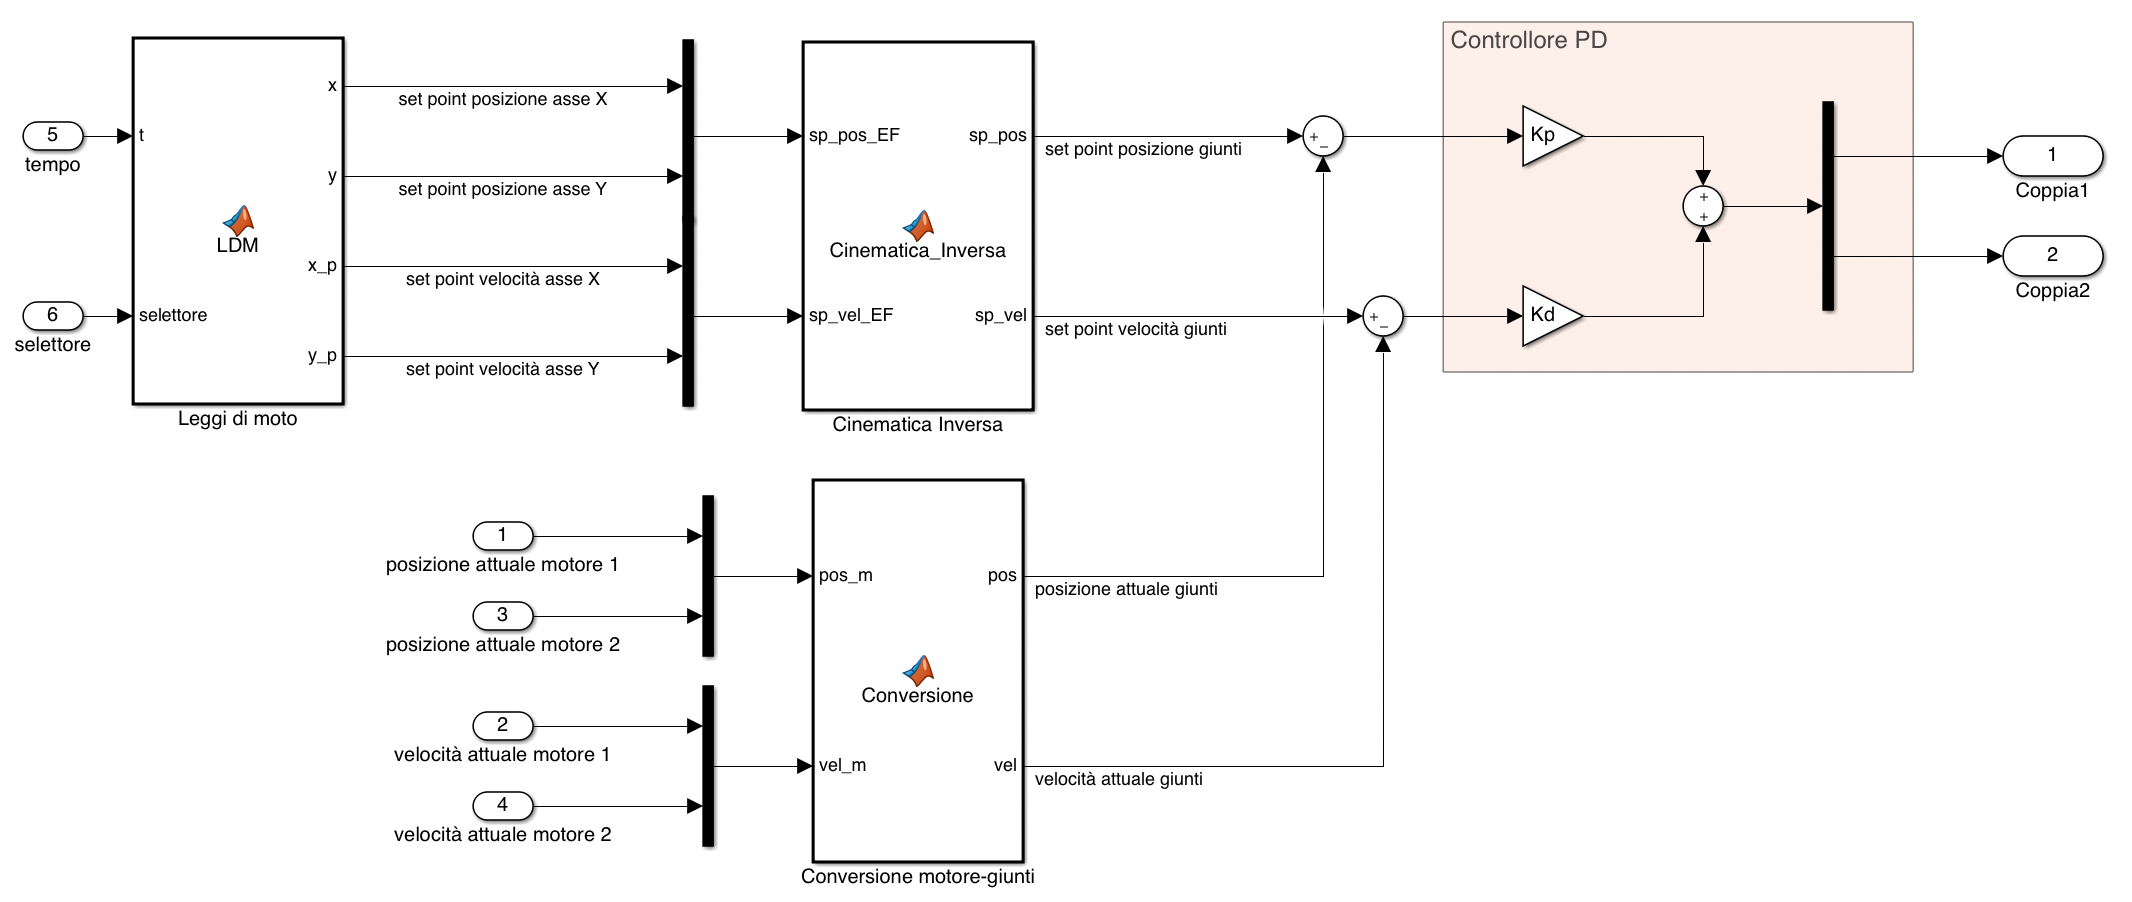
\includegraphics[scale=0.37]{Immagini/Controllori/PDBraccia}
		\caption{Controllore PD braccia}
		\label{fig:PDBraccia}
	\end{center}
\end{figure}
Avendo la possibilità di scegliere tra più traiettorie, a partire dal tempo attuale e dalla traiettoria desiderata andiamo a definire una legge di moto che fornirà i \textit{set-point} in posizione, velocità all'end-effector. Per andare a convertire questi in coordinate ai giunti vi è un blocco che si occupa di fare la cinematica inversa. Vengono poi lette le posizioni e velocità attuali dei motori e verranno successivamente convertite ai giunti; adesso che abbiamo tutto a livello di giunti possiamo fare la differenza tra riferimento e reale ottenendo un errore in posizione e uno in velocità\footnote{gli errori sono dei vettori $[2x1]$ contenenti le due componenti relative ai due angoli $\theta_1, \theta_2$.}. Gli errori verranno moltiplicati per $K_p$ e $K_d$ per ottenere la legge di controllo che verrà assegnata ai motori.
\par Per poter andare a testare il controllore è stata assegnata una legge di moto che disegna un cerchio di raggio $5cm$ in 5 secondi. Andiamo ora a vedere le coppie assegnate ai giunti $\theta_1$ e $\theta_2$:
\begin{figure}[!ht]
\begin{subfigure}{.5\textwidth}
  \centering
  % include first image
  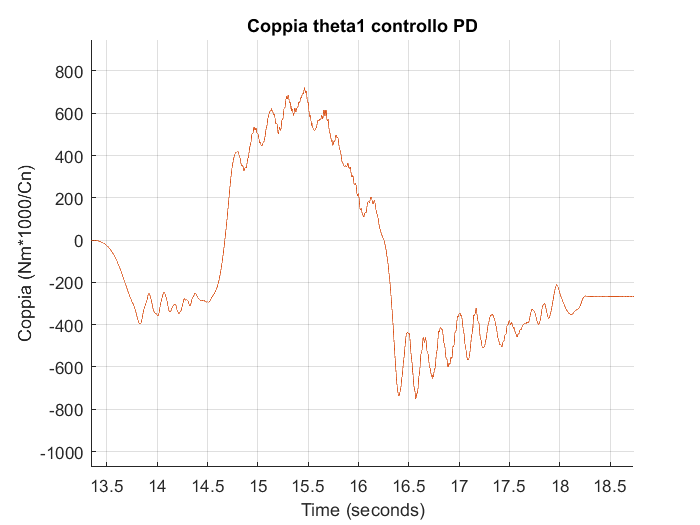
\includegraphics[width=.8\linewidth]{Immagini/Traiettorie/CoppiaT1PD}  
  \caption{Coppia $\theta_1$ controllore PD}
  \label{fig:sub-coppiaPD1}
\end{subfigure}
\begin{subfigure}{.5\textwidth}
  \centering
  % include second image
  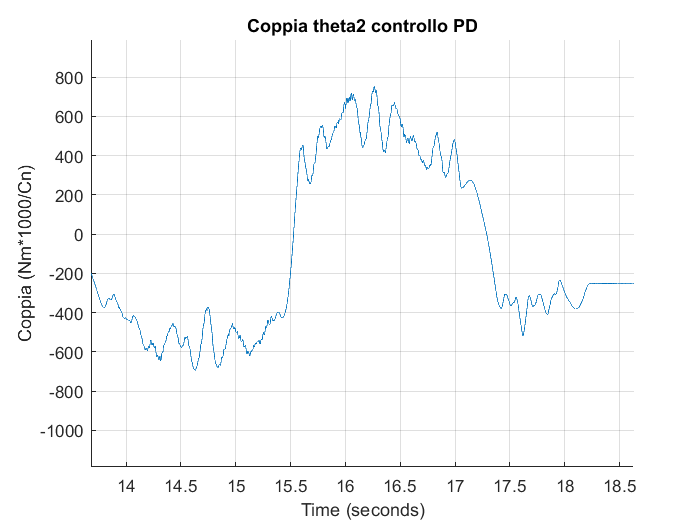
\includegraphics[width=.8\linewidth]{Immagini/Traiettorie/CoppiaT2PD}  
  \caption{Coppia $\theta_2$ controllore PD}
  \label{fig:sub-coppiaPD2}
\end{subfigure}
\caption{Coppie controllore PD braccia}
\end{figure}
Possiamo poi andare ad analizzare la posizione ottenuta con quelle coppie rispetto al riferimento, e di conseguenza possiamo guardare anche l'errore:
\begin{figure}[!ht]
\begin{subfigure}{.5\textwidth}
  \centering
  % include first image
  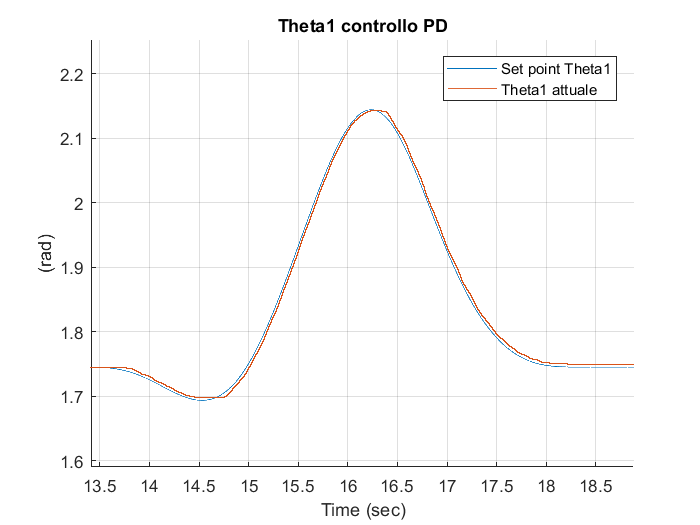
\includegraphics[width=.8\linewidth]{Immagini/Traiettorie/Theta1PD}  
  \caption{$\theta_1$ reale vs setpoint}
  \label{fig:sub-pd1p}
\end{subfigure}
\begin{subfigure}{.5\textwidth}
  \centering
  % include second image
  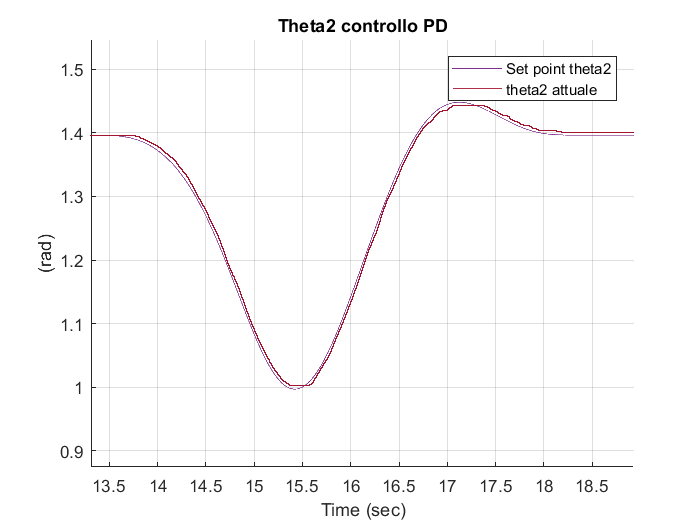
\includegraphics[width=.8\linewidth]{Immagini/Traiettorie/Theta2PD}  
  \caption{$\theta_2$ reale vs setpoint}
  \label{fig:sub-pd2p}
\end{subfigure}
\begin{subfigure}{.5\textwidth}
  \centering
  % include third image
  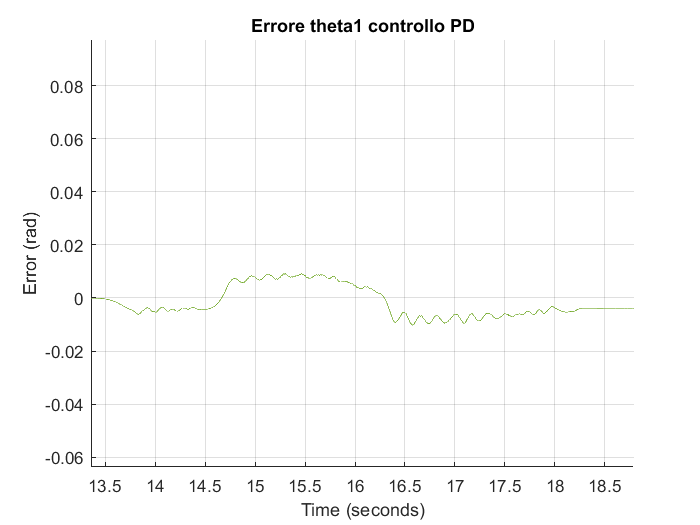
\includegraphics[width=.8\linewidth]{Immagini/Traiettorie/ErroreTheta1PD}  
  \caption{Errore su $\theta_1$}
  \label{fig:sub-pd3p}
\end{subfigure}
\begin{subfigure}{.5\textwidth}
  \centering
  % include third image
  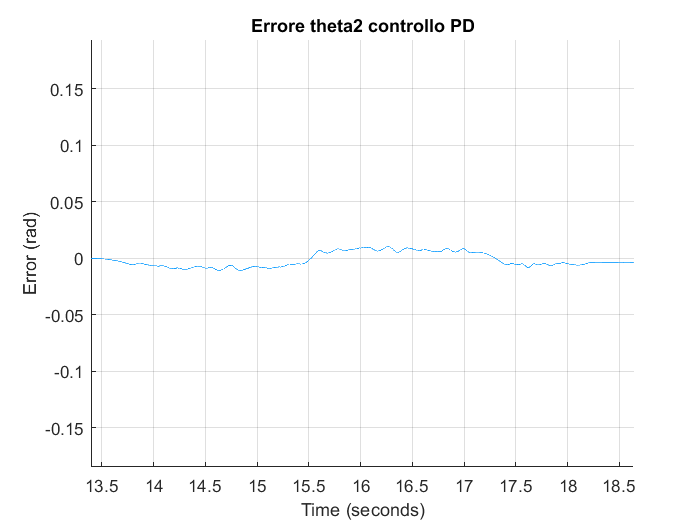
\includegraphics[width=.8\linewidth]{Immagini/Traiettorie/ErroreTheta2PD}  
  \caption{Errore su $\theta_2$}
  \label{fig:sub-pd4p}
\end{subfigure}
\caption{Andamenti posizione ed errori controllore PD}
\label{fig:AndamentiPD}
\end{figure}
Osservando i grafici si può notare che la posizione segue bene il setpoint andiamo poi a rappresentare la traiettoria reale e il riferimento anche sull'asse [X,Y] ottenendo: 
\begin{figure}[ht]
	\begin{center}
		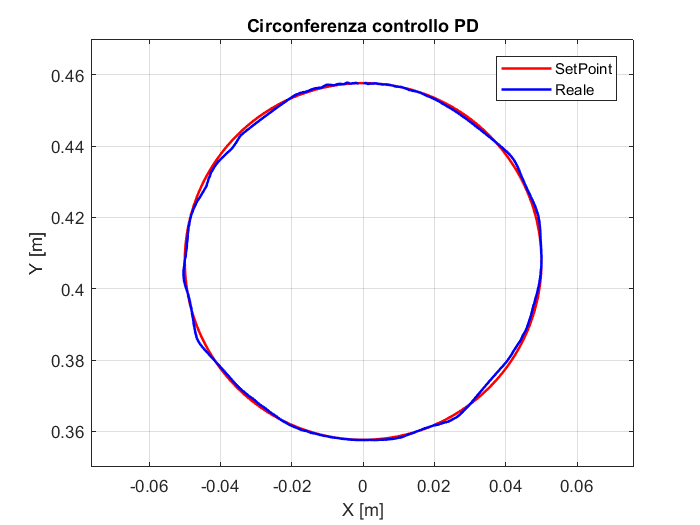
\includegraphics[scale=0.5]{Immagini/Traiettorie/Cerchio}
		\caption{Cerchio assi  [x,y] controllore PD}
		\label{fig:PDBracciaC}
	\end{center}
\end{figure}
[AGGIUNGI]
\subsubsection{Controllo feed-forward con coppia pre-computata}
Il passo successivo è stato quello di studiare ed implementare un controllore che opera in anello aperto; in particolare questo controllore calcola le coppie di disturbo basate sul modello matematico del sistema con parametri d'ingresso il \textit{set-point} in posizione e velocità e accelerazione. L'introduzione di questi termini riesce a risolvere in maniera corretta il problema del tracciamento della traiettoria desiderata, di conseguenza gli elementi introdotti riescono a compensare gli effetti di accoppiamento presenti nel modello dinamico del sistema. 
\begin{equation}
g_d = \Delta M(q^0_m)\ddot{q_m}^0 + C(q^0_m,\dot{q_m^0})\dot{q_m^0}
\end{equation}
L'idea è quindi che i termini vengono calcolati considerando i valori di posizione, velocità ed accelerazione del rifermento, in quanto mediante una legge di moto sono sempre ben noti. L'elemento $g_d$ compensa i termini di accoppiamento non lineari dovuti a forza d'inerzia, di Coriolis e centrifughe che dipendono dalla struttura e di conseguenza variano durante il movimento del manipolatore; in generale però calcolare questo termine è molto impegnativo, di conseguenza l'utilizzo di questo approccio su un sistema online può richiedere molto tempo, per questo solitamente vengono compensati solo i termini più importanti come quelli inerziali.
\begin{figure}[ht]
	\begin{center}
		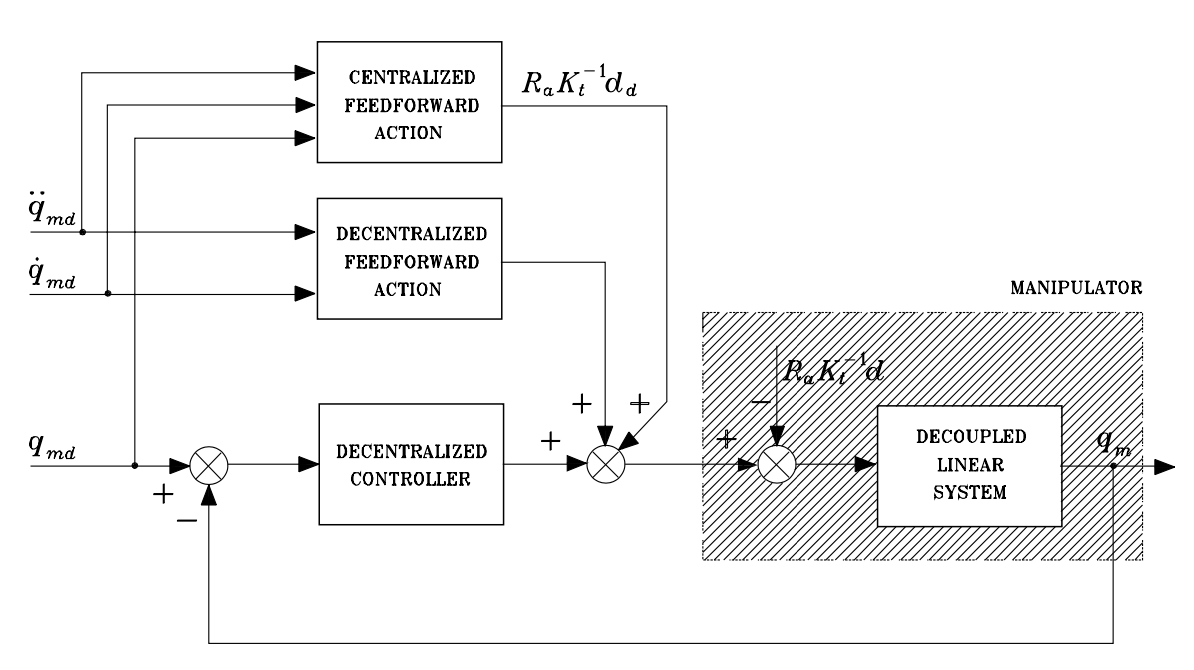
\includegraphics[scale=0.5]{Immagini/Controllori/FFschema}
		\caption{Schema teorico controllo feedforward}
		\label{fig:FFschema}
	\end{center}
\end{figure}
A livello implementativo possiamo vederlo come:
\begin{figure}[ht]
	\begin{center}
		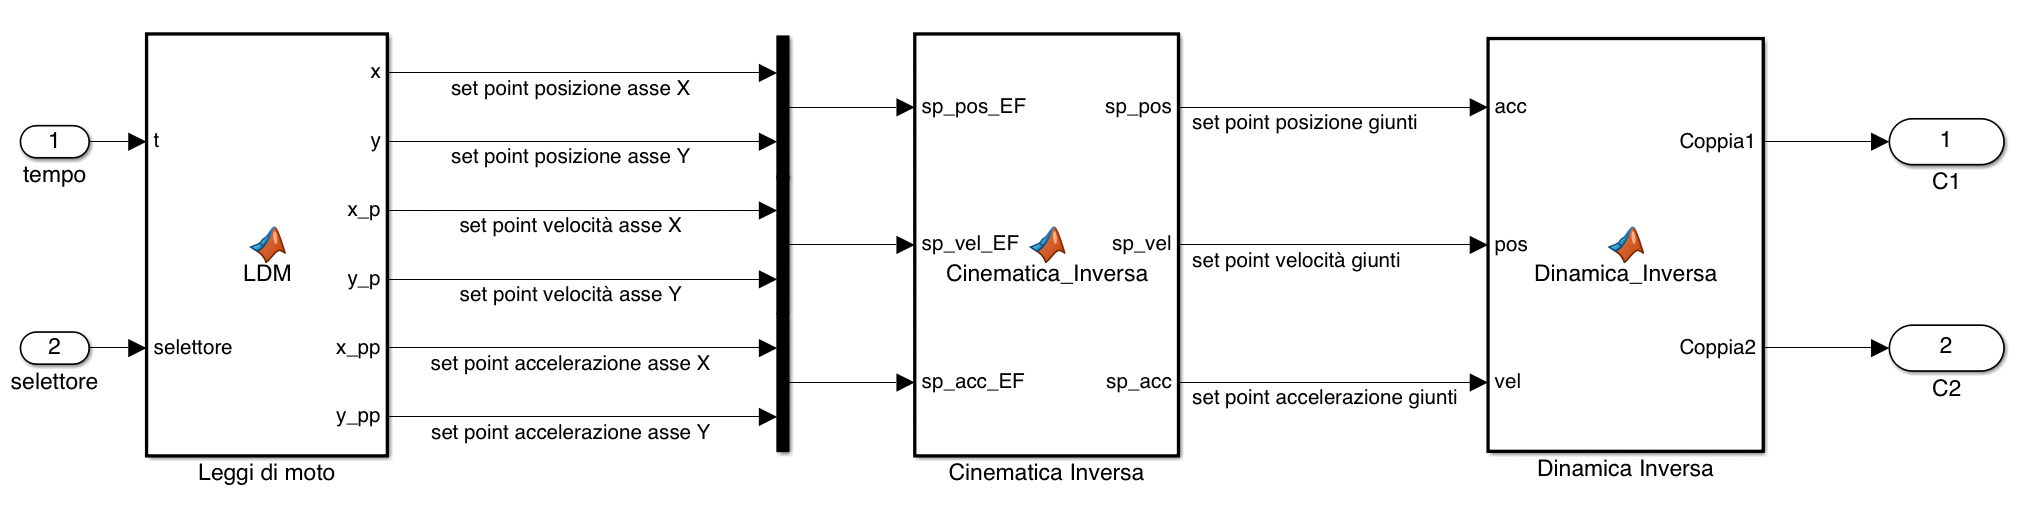
\includegraphics[scale=0.37]{Immagini/Controllori/feedForward}
		\caption{Controllore feedforward}
		\label{fig:FF}
	\end{center}
\end{figure}
\\A partire dalla legge di moto selezionata si ottengono i \textit{set-point} all'end-effector, che grazie alla cinematica inversa vengono convertiti in riferimento ai giunti.  Una volta ottenuti i riferimenti di posizione, velocità ed accelerazione si va ad applicare la funzione di dinamica inversa per calcolare le coppie di cui abbiamo bisogno. Le coppie sono quindi calcolate esclusivamente mediante dai riferimenti, è possibile vedere questo controllore come una versione di quello a dinamica inversa in anello aperto.
\begin{figure}
\begin{subfigure}{.5\textwidth}
  \centering
  % include third image
  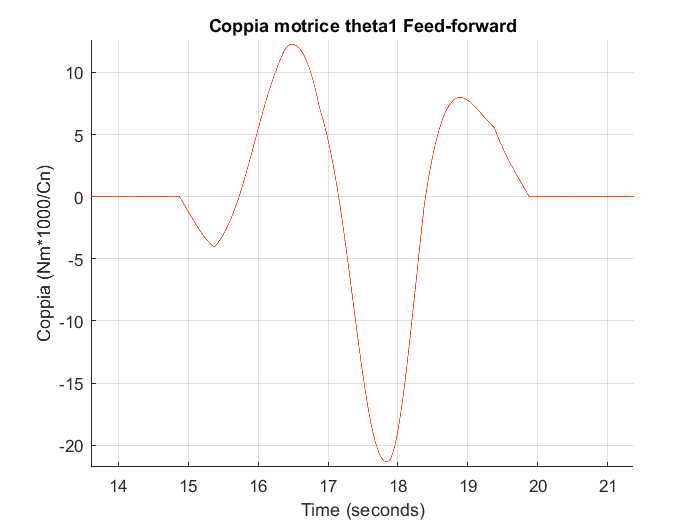
\includegraphics[width=.8\linewidth]{Immagini/Traiettorie/CoppiaT1FF}  
  \caption{Coppia $\theta_1$}
  \label{fig:sub-ff1}
\end{subfigure}
\begin{subfigure}{.5\textwidth}
  \centering
  % include third image
  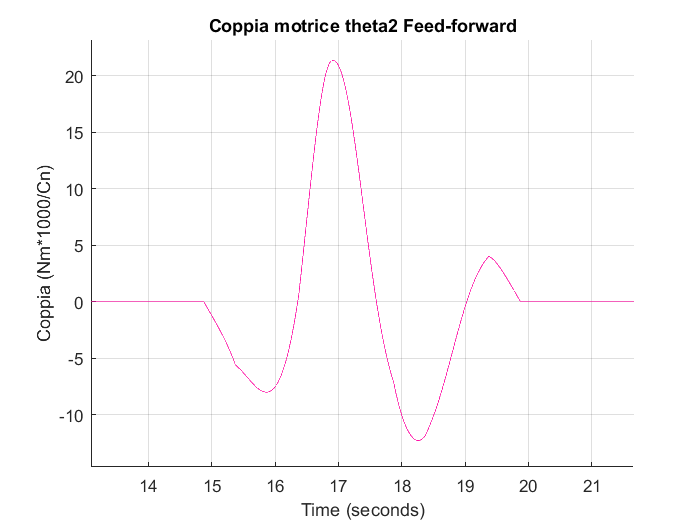
\includegraphics[width=.8\linewidth]{Immagini/Traiettorie/CoppiaT2FF}  
  \caption{Coppia $\theta_2$}
  \label{fig:sub-ff2}
\end{subfigure}
\caption{Coppie motori controllo fast-forward}
\label{fig:FFcoppie}
\end{figure}
\subsubsection{Controllo in dinamica inversa}
Riprendendo le tecniche di controllo centralizzato caratteristiche della letteratura l'approccio successivo è stato quello del controllo in dinamica inversa. Il primo step è stato quello di prendere l'equazione della dinamica e ridefinirla come: 
\begin{equation}
M(q_m)\ddot{q_m} + n(q_m,\dot{q_m}) = \tau_m
\label{eq:ControlloreID}
\end{equation}
Dove $n(q_m,\dot{q_m})$ raccoglie i termini centrifughi e di Coriolis (in letteratura raccoglie anche i termini gravitazionali, ma come anticipato precedentemente nel nostro caso equivalgono a zero). L'idea del controllo a dinamica inversa si basa sul trovare il vettore di coppie $\tau_m$ come funzione dello stato del sistema, cercando di creare una relazione ingresso-uscita di tipo lineare. Considerando che l'equazione della dinamica è lineare nel controllo e che la matrice d'inerzia è invertibile in ogni configurazione del manipolatore abbiamo la garanzia di trovare un controllore linearizzato di questo tipo. Possiamo andare a riscrivere il controllo come:
\begin{equation}
\tau_m = M(q_m)y + n(q_m,\dot{q_m})
\end{equation}
Dove $y = \ddot{q_m}$ rappresenta un vettore d'ingresso con espressione ancora da determinare. La legge di controllo è basata sul calcolo della dinamica inversa del manipolatore, il sistema è lineare e disaccoppiato rispetto al nuovo ingresso, questo implica che le componenti $y_k$ con $k = -\infty \dots m-1$ influenzano solo la variabile $q_m$ indipendentemente dal movimento degli altri giunti. In questo modo il problema del controllo è quello di trovare una legge \textbf{y} stabilizzante. Viene quindi scelta:
\begin{equation}
y = K_p\tilde{q} + K_d\tilde{\dot{q}}+\ddot{q}_m^0
\label{eq:yID}
\end{equation}
Dove con i termini $\tilde{q}$ e $\tilde{\dot{q}}$ si indica la differenza tra il \textit{setpoint} e la misurazione attuale di posizione e velocità. 
\begin{equation}
\tilde{q} = q^0_m - q_m \ \ \  \tilde{\dot{q}}= \dot{q}^0_m-\dot{q}_m
\label{eq:Tilde}
\end{equation}
Possiamo andare ora a sostituire le definizioni di \ref{eq:Tilde} in \ref{eq:yID} e troviamo l'espressione:
\begin{equation}
\tilde{\ddot{q}} + K_d + \tilde{\dot{q}} = 0
\end{equation}
Chiaramente l'errore si verifica quando uno o entrambi i termini sono diversi da zero.  Però, volendo assegnare la dinamica a ciascun giunto ci basta selezionare  i guadagni delle matrici $K_p$ e $K_d$ , inoltre, se le due matrici sono definite positive è possibile ottenere un sistema asintoticamente stabile. 
Possiamo scegliere le matrici come:
\begin{equation*}
K_p = diag(\omega^2_{01}, \dots, \omega^2_{0n}) \overline{M} \ \ \  K_d = diag(2 \xi_1 \omega_{01}, \dots ,2 \xi_n \omega_{0n}) \overline{M} 
\end{equation*}
Grazie al controllo a dinamica inversa i termini di compensazioni vengono calcolati ad ogni iterazione, quindi a piccoli intervalli temporali, il loop interno serve per ottenere una relazione ingresso/uscita lineare e disaccoppiata mentre quello esterno grazie alla dinamica desiderata serve a stabilizzare il sistema.
\begin{figure}[ht]
	\begin{center}
		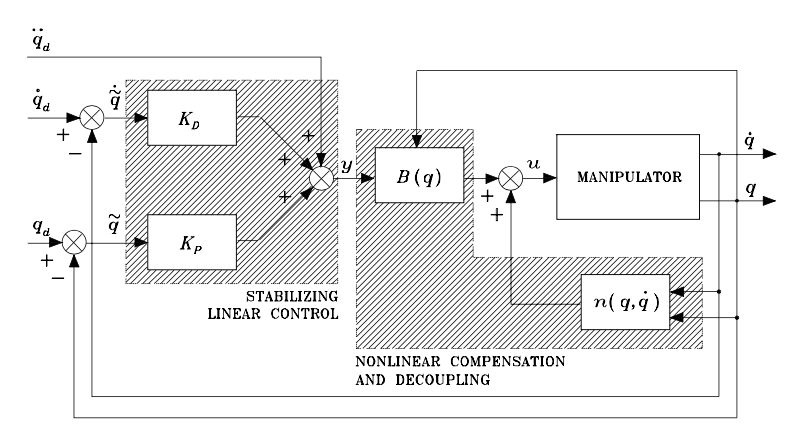
\includegraphics[scale=0.9]{Immagini/Controllori/IDTeoria}
		\caption{Schema controllore dinamica inversa}
		\label{fig:IDBraccia}
	\end{center}
\end{figure}
L'utilizzo di questo approccio è basato sull'ipotesi della cancellazione perfetta dei termini dinamici, quindi, i parametri dinamici del sistema devono essere accuratamente conosciuti e l'equazione del moto deve essere calcolata in real-time. Possiamo andare a vedere lo schema implementato sul controllore come:
\begin{figure}[ht]
	\begin{center}
		\includegraphics[scale=0.32]{Immagini/Controllori/SchemaID}
		\caption{Controllore dinamica inversa}
		\label{fig:IDRBraccia}
	\end{center}
\end{figure}
Come per tutti i controllori visti fino ad ora a partire da selettore e dal tempo ed applicando la cinematica inversa  andiamo ad ottenere i riferimenti di posizione,  velocità ed accelerazione; andiamo poi a prendere le posizioni e le velocità attuali dei motori e le convertiamo da motori ai giunti. Successivamente andiamo per posizione e velocità a trovare gli errori che verranno moltiplicati rispettivamente per $K_p$ e $K_d$. Per ottenere la y dobbiamo sommare questi due componenti insieme all'accelerazione del riferimento. Una volta ottenuto questo andiamo ad applicare la funzione di dinamica inversa con ingressi pari a $ID(y,q,\dot{q})$, da questa otteniamo la legge di controllo e le relative coppie che andranno assegnate ai link del manipolatore. 
\subsubsection*{Test Kp e Kd SISTEMARE}
\addcontentsline{toc}{subsubsection}{Test Kp e Kd}
Per andare a scegliere $K_p$ e $K_d$ in modo preciso è stato adottato un approccio sperimentale, ovvero far variare $K_p$, in un range di valori compreso tra 350 e 950 ad intervalli di 50, in base ad un valore fisso di $K_d$, il tutto facendo fare una traiettoria circolare ed andando ad analizzare quando il controllo iniziava a dar origine a vibrazione. Andiamo ora a vedere un risultato di questo metodo.
\begin{figure}[!ht]
\begin{subfigure}{.5\textwidth}
  \centering
  % include first image
  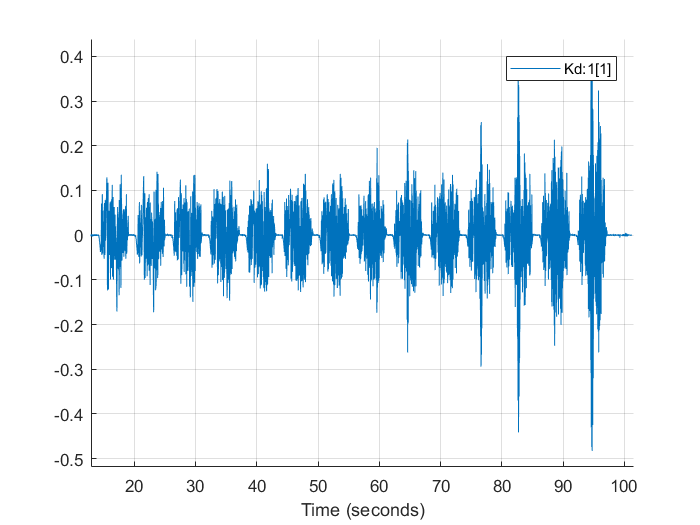
\includegraphics[width=.8\linewidth]{Immagini/Sperimentale/Test_Kd=15.png}  
  \caption{Test con $K_d$ = 1.5}
  \label{fig:sub-kd1.5}
\end{subfigure}
\begin{subfigure}{.5\textwidth}
  \centering
  % include second image
  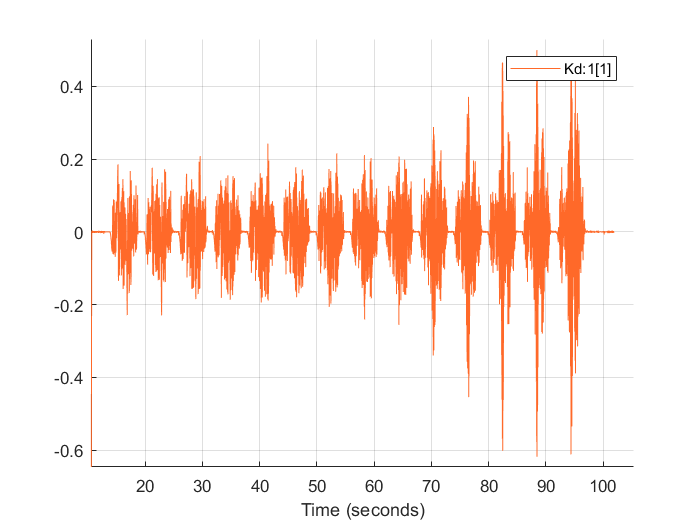
\includegraphics[width=.8\linewidth]{Immagini/Sperimentale/Test_Kd=2.png}  
  \caption{Test con $K_d$=2}
  \label{fig:sub-kd2}
\end{subfigure}
\begin{subfigure}{.5\textwidth}
  \centering
  % include third image
  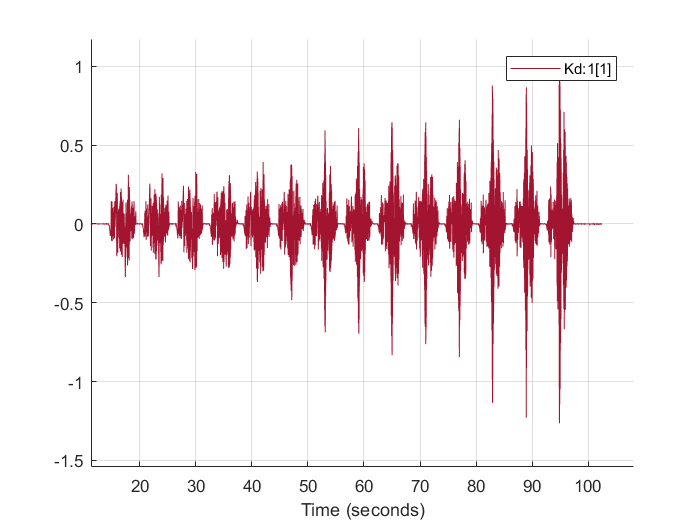
\includegraphics[width=.8\linewidth]{Immagini/Sperimentale/Test_Kd=3.png}  
  \caption{Test con $K_d$=3}
  \label{fig:sub-kd3}
\end{subfigure}
\begin{subfigure}{.5\textwidth}
  \centering
  % include third image
  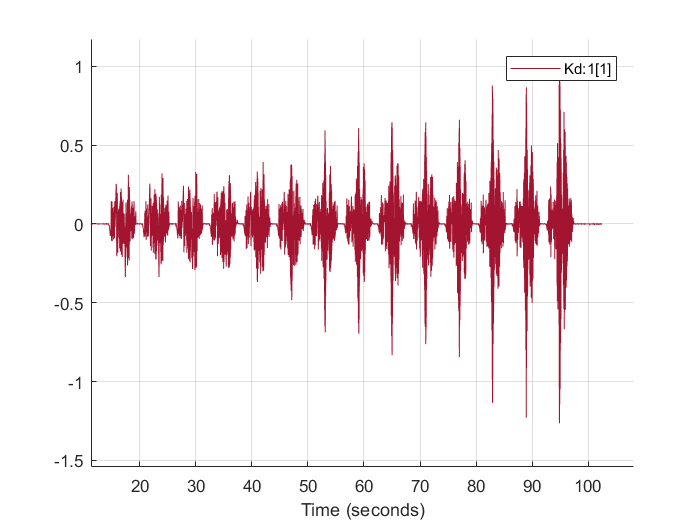
\includegraphics[width=.8\linewidth]{Immagini/Sperimentale/Test_Kd=3.png}  
  \caption{Test con $K_d$=3}
  \label{fig:sub-kd1}
\end{subfigure}
\caption{Test su $K_d$}
\label{fig:KdTest}
\end{figure}
\subsubsection*{Analisi}
Anche in questo caso, come nei precedenti la traiettoria principale testata è stata quella del cerchio raggio 5cm in 5 secondi, possiamo andare a vedere le coppie fornite ai giunti:
\begin{figure}
\begin{subfigure}{.53\textwidth}
  % include third image
  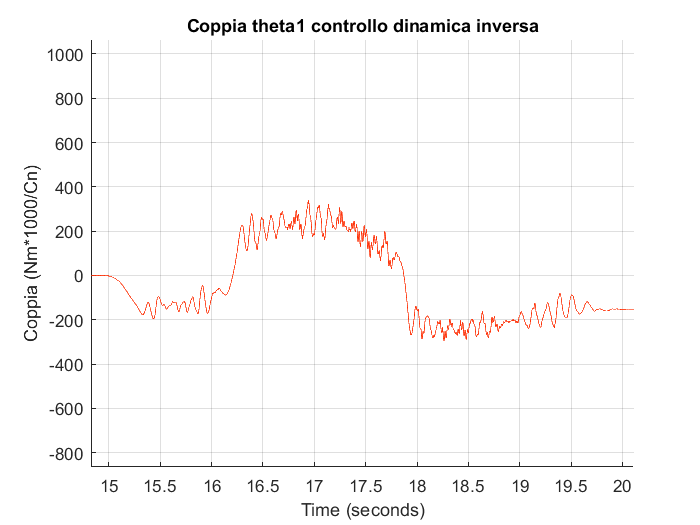
\includegraphics[width=.8\linewidth]{Immagini/Traiettorie/CoppiaT1ID}  
  \caption{Coppia $\theta_1$}
  \label{fig:sub-ikd1}
\end{subfigure}
\begin{subfigure}{.53\textwidth}
  % include third image
  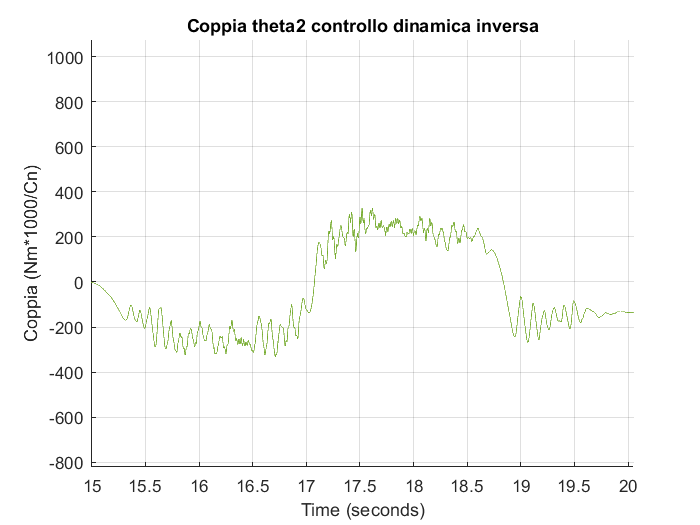
\includegraphics[width=.8\linewidth]{Immagini/Traiettorie/CoppiaT2ID}  
  \caption{Coppia $\theta_2$}
  \label{fig:sub-ikd2}
\end{subfigure}
\caption{Coppie giunti controllo dinamica inversa}
\label{fig:CoppieID}
\end{figure}
Come per il controllore PD possiamo andare a vedere e comparare la posizione attuale rispetto al riferimento e di conseguenza l'errore:
\begin{figure}[!ht]
\begin{subfigure}{.53\textwidth}
  \centering
  % include first image
  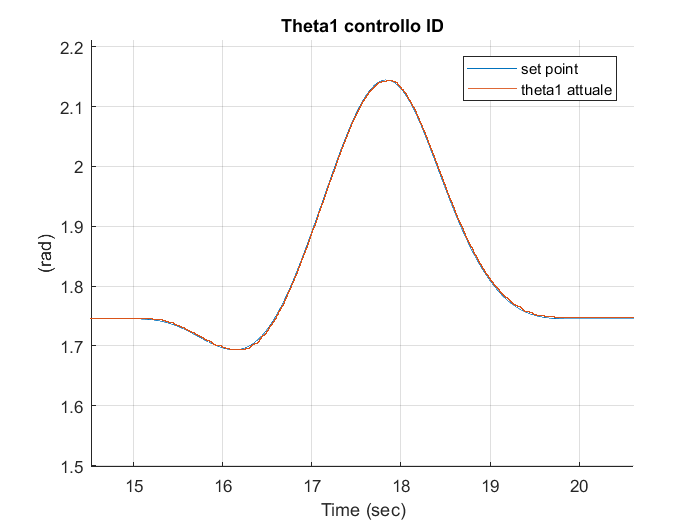
\includegraphics[width=.8\linewidth]{Immagini/Traiettorie/Theta1ID}  
  \caption{$\theta_1$ reale vs setpoint}
  \label{fig:sub-id1}
\end{subfigure}
\begin{subfigure}{.53\textwidth}
  \centering
  % include second image
  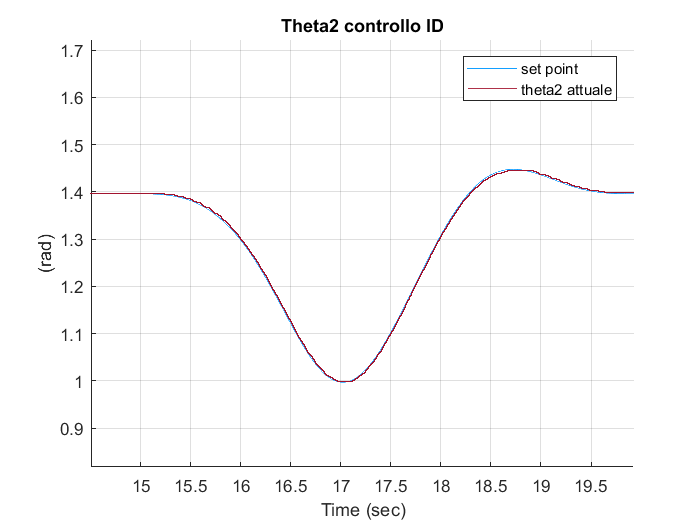
\includegraphics[width=.8\linewidth]{Immagini/Traiettorie/Theta2ID}  
  \caption{$\theta_2$ reale vs setpoint}
  \label{fig:sub-pd2k}
\end{subfigure}
\caption{Posizione vs riferimento controllore ID}
\end{figure}
\begin{figure}
\begin{subfigure}{.53\textwidth}
  \centering
  % include third image
  \includegraphics[width=.8\linewidth]{Immagini/Traiettorie/ErroreTheta1ID}  
  \caption{Errore su $\theta_1$}
  \label{fig:sub-pd3k}
\end{subfigure}
\begin{subfigure}{.5\textwidth}
  \centering
  % include third image
  \includegraphics[width=.8\linewidth]{Immagini/Traiettorie/ErroreTheta2ID}  
  \caption{Errore su $\theta_2$}
  \label{fig:sub-pd4}
\end{subfigure}
\caption{Errori controllore ID}
\label{fig:AndamentiID}
\end{figure}
Come per il controllore PD anche qua possiamo andare a rappresentare la traiettoria nel piano cartesiano, ottenendo:
\begin{figure}[ht]
	\begin{center}
		\includegraphics[scale=0.5]{Immagini/Traiettorie/CerchioDinamicaInversa}
		\caption{Cerchio [X,Y] controllo ID}
		\label{fig:IDbracciaC}
	\end{center}
\end{figure}
AGGIUNGI COMMENTI
\subsubsection{Controllo robusto}
 L'effetto di incertezze sul modello induce in errore il sistema di controllo, soprattutto nel caso reale bisogna supporre che la compensazione del modello dinamico risulti imperfetta magari a causa di approssimazioni oppure per semplificazioni.  Possiamo andare quindi a riscrivere l'equazione \ref{eq:ControlloreID} come:
\begin{equation}
\tau_m = \hat{M}(q_m)y + \hat{n}(q_m,\dot{q}_m)
\end{equation}
Dove $\hat{M}$ e $\hat{n}$ rappresentano i parametri stimati del modello dinamico, è possibile rappresentare l'incertezza come:
\begin{equation*}
\overline{M} = \hat{M}- M \ \ \overline{n} = \hat{n} - n
\end{equation*}  
Riprendendo la legge di controllo vista prima possiamo riscriverla come:
\begin{equation}
M(q_m)\ddot{q}_m + n(q_m,\dot{q_m}) = \hat{M}(q_m)y + \hat{n}(q_m,\dot{q_m})
\end{equation}
Essendo la matrice M invertibile in ogni configurazione possiamo ricavare $\ddot{q}_m$:
\begin{equation*}
\ddot{q}_m = y + (M^{-1}\hat{M}-I)y+M^{-1}\tilde{n} = y-\eta
\end{equation*}
Dove $\eta$ è una funzione non lineare definita come: \begin{equation}
\eta = (I-M^{-1}\hat{M})y - M^{-1}\tilde{n} 
\end{equation}
Adottando la legge \ref{eq:Tilde} vista nel caso del controllore a dinamica inversa possiamo ottenere che l'errore dinamico è gestito dall'equazione:
\begin{equation}
\ddot{\tilde{q}} + K_d \dot{\tilde{q}} + K_p\tilde{q} = \eta
\end{equation}
Otteniamo quindi un sistema non lineare e accoppiato, di conseguenza implementare un semplice controllore PD non basta; per risolvere questo problema occorre inserire un termine non lineare, che sia funzione dell'errore e creato appositamente per fornire robustezza al controllo. Come per il controllore PD si ricerca una funzione grazie al metodo diretto di Lyapunov. 
Andiamo a definire lo stato del sistema come:
\begin{equation*}
\xi = \begin{bmatrix}
\tilde{q} \\ \dot{\tilde{q}}
\end{bmatrix}
\end{equation*}
sostituendo poi lo stato nell'equazione $\ddot{q}_m = y-\eta$ si ottiene un'equazione differenziale del primo ordine
\begin{equation}
\dot{\xi} = H\xi + D(\ddot{q}_m^0 - y + \eta)
\end{equation}
Dove H e D sono definite come:$H = \begin{bmatrix}
0 & I \\ 0 & 0
\end{bmatrix} \in \mathbb{R}^{(2nx2n)}$ , $D = \begin{bmatrix}
0 \\ I
\end{bmatrix} \in \mathbb{R}^{(2nxn)}$
\\Si può vedere il problema di inseguimento della traiettoria come la soluzione che va a stabilizzare il sistema non lineare di qui sopra. Nella letteratura del controllore robusto, anche se l'incertezza $\eta$ non è nota è comunque disponibile un suo intervallo di variazione. La legge \textbf{y} dovrebbe garantire stabilità di $\dot{\xi}$ per ogni $\eta$ nell'intervallo. Di conseguenza vengono formulate tre assunzioni:
\begin{enumerate}
\item $\sup_{t\ge 0} ||\ddot{q}^0_m || < Q_M < \infty \forall \ddot{q}_m^0$
\item $||I-M^{-1}\hat{M}(q_m)|| \le \alpha \le 1 \forall q_m$
\item $||\tilde{n}|| \le \Phi(||\xi||) < \infty \forall q_m, \dot{q}_m$
\end{enumerate}
Andando ad analizzare le assunzioni possiamo dire che:
\begin{itemize}
\item La prima assunzione è soddisfatta sempre, in quanto per ogni traiettoria definita le accelerazioni non possono essere infinite
\item La seconda assunzione conferma che M  (e di conseguenza $M^{-1}$) sia superiormente e inferiormente limitata, infatti 
\begin{equation}
0 < M_m < ||M^{-1}(q_m)|| \le M_M < \infty \forall q_m
\end{equation}
\end{itemize}
Quindi, esiste sempre una scelta di $\hat{M}$ che soddisfa la condizione, selezionando per esempio
\begin{equation*}
\hat{M} = \frac{2}{M_M+M_m}I
\end{equation*} 
otteniamo
\begin{equation}
||M^{-1}(q_m)\hat{M}(q_m)-I|\le \alpha = \frac{M_M-M_m}{M_M+M_m} <1
\end{equation}
Il limite inferiore si ha quando $\hat{M} = M$ in quanto $\alpha = 0$. Concentrandoci sull'assunzione 3, si può osservare che $\tilde{n}$ è funzione di $q_m,\dot{q_m}$, nel primo caso, in base alla tipologia di giunto (rotoidale o prismatico) abbiamo intervalli che sono limitati e quindi il contributo è limitato. Anche la velocità è limitata grazie all'effetto della saturazione (esistente sulle velocità massime dei motori). Di conseguenza, prendiamo per $\Phi$ una funzione calcolata nella norma dello stato come:
\begin{equation}
\Phi(||\xi||) = \alpha_0 + \alpha_1 ||\xi|| + \alpha_2 ||\xi||^2
\end{equation}
Andando a riprendere la legge di controllo\ref{eq:yID} ed ampliandola possiamo definirla come: 
\begin{equation}
y = \ddot{q}^0_m + K_p\tilde{q} + K_d\dot{\tilde{q}} + \omega
\label{eq:yRob}
\end{equation}
Il termine PD ci assicura la stabilizzazione della dinamica della matrice dell'errore, $\ddot{q}^0_m$ fornisce un termine di previsione e $\omega$ è progettato in modo da combattere l'incertezza fornendo robustezza al sistema.
\begin{equation}
\dot{\xi} = \tilde{H}\xi + D(\eta-\omega)
\end{equation}
Dove:
\begin{equation*}
\tilde{H} = H-DK = \begin{bmatrix}
0 & I \\ -K_p & -K_d
\end{bmatrix} \in 
\mathbb{R}^{(2nx2n)}
\end{equation*}
\begin{equation*}
 \ K_p = diag(\omega^2_{01}, \dots, \omega^2_{0n})  \ \ \  K_d = diag(2 \xi_1 \omega^2_{01}, \dots ,2 \xi_n \omega^2_{0n}) 
\end{equation*}
Per andare a definire $omega$ si procede col metodo diretto di Lyapunov; consideriamo come funzione:
\begin{equation}
V(\xi) = \xi^TQ\xi >0 , \forall \xi \neq 0
\end{equation}
con Q matrice simmetrica definita positiva. Facendo la derivata lungo la traiettoria si trova che
\begin{equation}
\dot{V} = \xi^T P\xi + 2z^T(\eta-\omega)
\label{eq:LyapDerivRob}
\end{equation}
Considerando che $\tilde{H}$ ha tutti gli autovalori con parte reale negativa, possiamo scegliere una qualunque P definita positiva che soddisfi:
\begin{equation*}
\tilde{H}^TQ+Q\tilde{H} = -P
\end{equation*}
Consideriamo ora l'equazione \ref{eq:LyapDerivRob} , $z = D^TQ\xi$, il primo termine sulla parte di destra è definito negativo, di conseguenza la soluzione converge solo se $\xi \in \mathbb{N}(D^TQ)$, se invece non appartiene, il controllo $\omega$ andrà scelto per rendere il secondo termine minore o uguale a zero utilizzando la legge di controllo:
\begin{equation}
\omega = \rho(||\xi||)\frac{z}{||z||}, \rho >0
\end{equation}
con $\rho$ funzione positiva da determinare. Scegliendo $\omega$ in questo modo otteniamo:
\begin{equation*}
z^T(\eta-\omega) = z^T\eta - \rho(||\xi||)\frac{zz^T}{||z||} \le ||z||\big[||\eta||.\rho(||\xi||)\big]
\end{equation*}
se poi garantiamo che: $||\xi||>||\eta||$ per ogni valore di posizione, velocità e velocità di riferimento, otteniamo che questo termine e $\dot{V}$ sono negativi lungo tutte le traiettorie dell'errore; per poter soddisfare la disuguaglianza, dalla definizione di $\eta$ troviamo:
\begin{equation}
\eta = (I-M^{-1}\hat{M})y-M^{-1}\tilde{n} \ e \ y = \ddot{q}^0_m + K\xi+\omega
\end{equation}
sapendo poi che $||\omega|| = \rho$ troviamo che:
\begin{equation*}
||\eta|| \le ||I-M^{-1}\hat{M}|| (||\ddot{q}_m^0 ||+||K||\  ||\xi||+||\omega||)+||M^{-1}|| \ ||\tilde{n}||
\end{equation*}
Andando a maggiorare questa quantità troviamo che:
\begin{equation}
||\eta|| \le \alpha Q_M + \alpha ||K|| || \xi || + \alpha\rho(||\xi||)+M_M\Phi(||\xi||) < \rho(||\xi||)
\end{equation}
è quindi possibile andare a selezionare un $rho$ in modo tale che:
\begin{equation}
\rho(||\xi||) \ge \frac{1}{1-\alpha} [\alpha Q_M+\alpha ||K|| ||\xi||+M_M\Phi(||\xi||)]
\label{eq:HelpRho}
\end{equation}
Si può osservare che $\Phi(||\xi||) = \alpha_0+\alpha_1||\xi||+\alpha_2||\xi||^2$ per soddisfare \ref{eq:HelpRho} basta che si selezionino:
\begin{equation*}
\rho(||\xi||) = \beta_0 + \beta_1||\xi||+\beta_2||\xi||^2
\end{equation*}
Con i valori:
\begin{equation*}
\begin{cases}
\beta_0 \ge \frac{\alpha Q_M+\alpha_0M_M}{1-\alpha}\\
 \beta_1 \ge \frac{\alpha K +\alpha_1 M_M}{1-\alpha}\\
 \beta_2 \ge \frac{\alpha_2M_M}{1-\alpha}
\end{cases}
\end{equation*}
Andando poi a sostituire tutto nell'equazione \ref{eq:LyapDerivRob} troviamo:
\begin{equation}
\dot{V} = -\xi^T P \xi + 2z^T(\eta-\rho(||\xi||) \frac{z}{||z||}) <0 \ \forall
\xi \neq 0
\end{equation}
Di conseguenza $\xi = 0$ è un equilibrio di stato asintoticamente e globalmente stabile. La legge di controllo è quindi formata da tre termini, un primo termine che compensa i termini non lineari e gli accoppiamenti tra i link, un secondo terine che stabilizza il sistema dinamico grazie ad una retroazione con previsione per l'errore e un terzo termine che fornisce robustezza contrastando le incertezze e calcolando i termini non lineari che dipendono dallo stato del manipolatore. 
\par Ad alte frequenze però potrebbe esserci la commutazione della variabile di controllo, che potrebbe portare ad un'elevata presenza di "sali/scendi" a causa del terzo termine, per questo possiamo approssimarlo come:
\begin{equation}
\omega = \begin{cases}
\rho(||\xi||) \frac{z}{||z||} \ for\ ||z||\ge \varepsilon \\
\rho(||\xi||) \frac{z}{\varepsilon} \ \ \ for \ ||z|| < \varepsilon
\end{cases}
\end{equation}
Possiamo andare quindi a rappresentare lo schema del controllo robusto teorico nel seguente modo:
\begin{figure}[ht]
	\begin{center}
		\includegraphics[scale=0.8]{Immagini/Controllori/RobustTeoria}
		\caption{Schema controllore robusto}
		\label{fig:RobustSchema}
	\end{center}
\end{figure}
Data la difficoltà implementativa del controllore robusto sul modello reale sono state condotte due tipologie di analisi: la prima è stata un'analisi del comportamento del controllore grazie alla modellazione di un sistema più semplice, in particolare il sistema ad un grado di libertà del manovellismo; la seconda invece è stata la simulazione del controllore sul modello simulink del manipolatore.
\subsubsection*{Analisi manovellismo}
\addcontentsline{toc}{subsubsection}{Analisi manovellismo}
Come è stato anticipato precedentemente è stata fatta un'analisi mediante il sistema ad un grado di libertà biella manovella, 
\begin{figure}[ht]
	\begin{center}
		\includegraphics[scale=0.6]{Immagini/Sperimentale/BiellaManovella}
		\caption{Sistema biella manovella}
		\label{fig:BiellaManovella}
	\end{center}
\end{figure}
[PRESENTA RISULTATI]
\subsection{Confronto approcci controllori}
Avendo introdotto e verificato le principali tipologie di controllo centralizzato è venuto il momento di fare un confronto andando a vedere quale tra gli approcci visti è il migliore. In particolare, sulla traiettoria effettuata andiamo a confrontare gli errori tra il controllore PD e quello ID:
\begin{figure}[!ht]
\begin{subfigure}{.53\textwidth}
  \centering
  % include first image
  \includegraphics[width=.8\linewidth]{Immagini/Traiettorie/ConfontoErroriTheta1}  
  \caption{Confronto errore $\theta_1$ }
  \label{fig:sub-tid1}
\end{subfigure}
\begin{subfigure}{.53\textwidth}
  \centering
  % include second image
  \includegraphics[width=.8\linewidth]{Immagini/Traiettorie/ConfontoErroriTheta2}  
  \caption{Confronto errore $\theta_2$}
  \label{fig:sub-tid2}
\end{subfigure}
\caption{Confronto controllore PD e ID}
\end{figure}
Da entrambe le immagini è chiaro come è il controllore a dinamica inversa a prevalere. Di conseguenza si è scelto questo come controllore definitivo e sono stati analizzati altri andamenti con leggi di moto diverse per valutare il comportamento del controllore.
\begin{figure}[ht]
	\begin{center}
		\includegraphics[scale=0.4]{Immagini/Traiettorie/QuadratoDinamicaInversa}
		\caption{Quadrato controllo dinamica inversa}
		\label{fig:quadID}
	\end{center}
\end{figure}
\begin{figure}[ht]
	\begin{center}
		\includegraphics[scale=0.4]{Immagini/Traiettorie/PatternDinamicaInversa}
		\caption{Pattern controllo dinamica inversa}
		\label{fig:patternID}
	\end{center}
\end{figure}
\subsubsection{Filtro di Kalman}